% Chapter Template

\chapter{Estructura del mutualismo} % Main chapter title
\label{ChapterESTATICA}  % Change X to a consecutive number; for referencing this chapter elsewhere, use \ref{ChapterX}


En el capítulo anterior se ha descrito como la estructura de la red mutualista determina su dinámica de poblaciones. El conjunto de interacciones es la trama que sostiene la biodiversidad de los ecosistemas \cite{mccann2007protecting}.
Las propiedades de las redes se resumen mediante indicadores estadísticos globales como el \textit{anidamiento}
y la \textit{modularidad}. Por su parte las medidas locales de centralidad y grado permiten ordenar las especies y conocer su importancia relativa para la resistencia de la red ante perturbaciones externas. 

Los índices que se manejan en la literatura son numerosos y de origen diverso y no existe un marco teórico que explique de manera inequívoca las relaciones entre los observables más habituales.

En este capítulo se describe el potencial de una técnica clásica en el análisis de grafos, conocida como \textit{descomposición k-core}, en el estudio de las redes mutualistas.

%----------------------------------------------------------------------------------------
%	SECTION 1
%----------------------------------------------------------------------------------------

\section{Propiedades estructurales del mutualismo}
\label{sec:prop_mutualismo}

Como se indicó en la introducción, la investigación sobre la estructura del mutualismo heredó las herramientas conceptuales del análisis de las \textit{food webs}, entre ellas el uso de la \textit{conectancia}. Esta magnitud es la fracción de enlaces presentes sobre todos los posibles entre las especies de ambas clases. Resulta un índice global de utilidad limitada, pero sigue
usándose para la construcción de modelos nulos que veremos en este mismo capítulo. La distribución de grado es la traducción local de la conectancia,
y es muy heterogénea en las redes mutualistas, con algunas especies mucho más conectadas de lo que cabría esperar por azar \cite{jordano2003invariant}.

Durante la última década el \textit{anidamiento} se ha considerado como la característica distintiva del mutualismo \cite{bascompte2003nested}, aunque en la actualidad esta afirmación está sujeta a revisión. Este concepto tiene una definición clara en ecología, una comunidad es anidada si las especies encontradas en un ámbito geográfico reducido son un subconjunto de las existentes en un ámbito mayor más rico en recursos. Originalmente se aplicó al estudio de la distribución de la fauna en islas. La de una isla pequeña es un subconjunto de la que existe en tierra firme o en una isla mayor de las mismas características biogeográficas \cite{young1958zoogeography, atmar1986nested}.

Si las especies se ordenan por grado, la matriz de interacción de una comunidad con anidamiento fuerte muestra abundancia de interacciones entre las especies situadas en el vértice superior izquierdo. Allí se concentran las muy conectadas,
las de grado reducido aparecen conectadas con este núcleo y raramente entre ellas.

En las redes mutualistas se observa un grupo de especies generalistas con un alto número de conexiones y especialistas que se conectan con las generalistas pero apenas con otras especialistas. Esta organización, que tradicionalmente se ha caracterizado como anidamiento, parece proporcionar estabilidad estructural y maximizar las poblaciones de la comunidad \cite{memmott2004tolerance,bastolla2009,thebault2010stability,suweis2013emergence}. 

La medida del anidamiento es la más popular en el análisis del mutualismo, pero no está exenta de problemas. El principal es que existen distintos indicadores que no son equivalentes. No vamos a hacer una revisión de todos ellos, porque la producción en este terreno ha sido prolífica \cite{ulrich2009consumer}, pero mencionaremos los más destacados. 

Los basados en la \textit{temperatura} comparan la posición de los elementos de la matriz de interacción con la llamada isoclina de anidamiento perfecto. La curvatura de esta línea se define por conectancia de la red. La temperatura se calcula con una función del número enlaces por debajo de la isoclina o los huecos por encima de ella y de la distancia a la que se encuentran de esta \cite{ulrich2007null}. El método más popular es el \textit{Nestedness Temperature Calculator}(N TC) de Atmar y Patterson \cite{atmar1995nestedness}.

Los métodos de tipo \textit{gap} se basan en un conteo del número de veces que habría que mover los enlaces de la matriz para conseguir un anidamiento perfecto. El primero en publicarse fue el llamado $BR$ \cite{brualdi1999nested}.

La tercera aproximación consiste en utilizar la definición original de anidamiento y medir la superposición (\textit{overlaping}). Se cuentan las interacciones por filas y columnas y se identifican las que son subconjuntos por similaridad. El primer índice en seguir este criterio fue el $HH$ \cite{hausdorf2003nestedness}. En los últimos años se han empleado mucho evoluciones de esta idea como $NODF$ (\textit{Node Overlap Decreasing Fill}) \cite{almeida2008consistent} y $PRN$ (\textit{Percentage Relativized Nestedness}) \cite{podani2012comparative}.

En los métodos descritos la matriz de interacción es binaria, o se trata como tal. Si se desea tener el cuenta el peso de los enlaces, en el
caso de que se disponga de datos, existen alterantivas. $WNODF$ es una modificación de $NODF$ \cite{almeida2011straightforward}, mientras que $WIN$ se basa en la distancia Manhattan \cite{galeano2009weighted}. Por último, hay que citar el \textit{Radio Espectral} \cite{staniczenko2013ghost}. Este índice es el valor del módulo del autovalor máximo de la matriz de interacción, y es válido tanto para matrices binarias como pesadas. 

Otro indicador global que se emplea de forma habitual en la caracterización del mutualismo es la modularidad \cite{newman2004finding, olesen2007modularity}. De una forma intuitiva, los módulos son grupos de nodos fuertemente conectados entre sí dentro de una red con baja conectividad.
Al igual que sucede con el anidamiento, existen diferentes algoritmos para el cálculo de la modularidad. En mutualismo el
más usado es el de Barber para redes binarias \cite{barber2007modularity} y una versión reciente (\textit{QuanBiMo}) para redes pesadas \cite{dormann2014method}.

La relación entre modularidad y anidamiento en las redes mutualistas ha despertado el interés de la comunidad científica \cite{olesen2007modularity, dupont2009ecological}. Parecen comportarse como propiedades en cierto sentido antagónicas y por tanto como reguladoras de la estabilidad \cite{fortuna2010nestedness}. Por ejemplo, los módulos actúan como cortafuegos ante las extinciones en cascada \cite{saavedra2011strong} mientras que las redes muy anidadas son más vulnerables a este fenómeno \cite{lever2014sudden}. 

Ambas magnitudes se corresponden con propiedades globales de la red, pero no ofrecen medidas locales. No tiene sentido hablar de anidamiento o modularidad de una especie. Esta limitación supone un obstáculo en la práctica a la hora de definir políticas de conservación, porque no resultan útiles para predecir el comportamiento ante extinciones parciales. Desde un punto de vista analítico, también es deseable poder encontrar principios que funcionen tanto a escala global como a escala local. 
Además, la relación entre anidamiento, modularidad y establidad de la red es un tema de intenso debate académico \cite{fortuna2010nestedness, james2012disentangling, staniczenko2013ghost, feng2014heterogeneity}. Como resultado de todas estas consideraciones, la búsqueda de medidas alternativas, basadas en propiedades estadísticas o topológicas, es un campo de investigación muy activo \cite{podani2014new,chagnon2015characterizing,strona2015new}.

\section{Descripción basada en la descomposición \textit{k-core}}

La \textit{descomposición k-core}\footnote{Utilizamos la expresión original en inglés por ser prevalente en la bibliografía, a pesar de que algunos autores han propuesto traducciones como \textit{núcleos de grado k} \cite{herrero2000terminologia} o \textit{k-núcleos} \cite{cardona2006taxonomia, martinez2011aplicacion}} fue utilizada por primera vez por Stefen Seidman para medir la densidad local y la cohesión en redes sociales \cite{seidman1983network}. Dado un grafo no dirigido, un \textit{k-core} es el subgrafo máximo el el que todos sus nodos están conectados con al menos otros $k$ puntos \cite{dorogovtsev2006k}.

La \textit{descomposición k-core} se ha utilizado de forma habitual como mecanismo de reducción de información para estudiar redes de distinta naturaleza \cite{kitsak2010identification, zhang2010using, barbera2015critical}. El resultado ofrece una visión organizada en capas, con los nodos más centrales en la \textit{shell} de mayor $k$. Esta cifra puede llegar al orden de las centenas en redes grandes. Hasta donde nosotros sabemos, no hay literatura sobre su aplicación al estudio del mutualismo, ya que son redes bipartitas de un tamaño mínimo comparado con los sistemas sociales o tecnológicos a los que se ha aplicado.

\begin{theo} 
Sea un grafo no dirigido $G = \{V, E\}$, donde $V$ y $E$ son los conjuntos de nodos y enlaces respectivamente. Llamamos $deg_G(v)$ al grado del nodo $v$ en el grafo $G$. El subgrafo $M = \{C, E|C\}$ inducido por el subconjunto de nodos $C \subseteq V$ es
un $k$-$core$ si $\forall v \in C: \big( deg_G(v) \geq k \big)$ y $M$ es el subgrafo máximo que cumple la condición. Se denomina $k$-$shell$ al conjunto de nodos del $k$-$core$ que no pertenecen al \textit{$k+1$ core}.
\label{ESTATICA_def_kcore}
\end{theo}

Existen diversos algoritmos para llevar a cabo la descomposición en función de las dimensiones de la red \cite{montresor2013distributed}. El más sencillo y válido para el caso de las redes mutualistas es el algoritmo de podado (\textit{pruning}), que se describe con la ayuda de la figura \ref{fig:ESTATICA_kcore_decomposition_example}, una red bipartita ficticia, con ocho nodos de una clase y siete de la opuesta. A la hora de aplicar el algoritmo resulta irrelevante que la red sea bipartita, pues solo se basa en el número de enlaces y no en la naturaleza de los nodos que conectan.

Se empieza eliminando enlaces de aquellos nodos que solo tienen uno, por ejemplo el que une el nodo de color verde número 8 con el de color chocolate número 4. Se repite la operación mientras queden nodos con un único enlace, hasta que llegue el momento en que todos los nodos restantes tengan dos o más. Los nodos que han quedado desconectados forman la \textit{1-shell}. Repetimos el procedimiento para dos enlaces y así sucesivamente, clasificando todos los nodos en su \textit{shell} correspondiente. En este ejemplo sencillo el $k$ máximo es 3. Nótese que cada nodo pertenece a una $shell$.

\begin{figure}[h!]
\centering
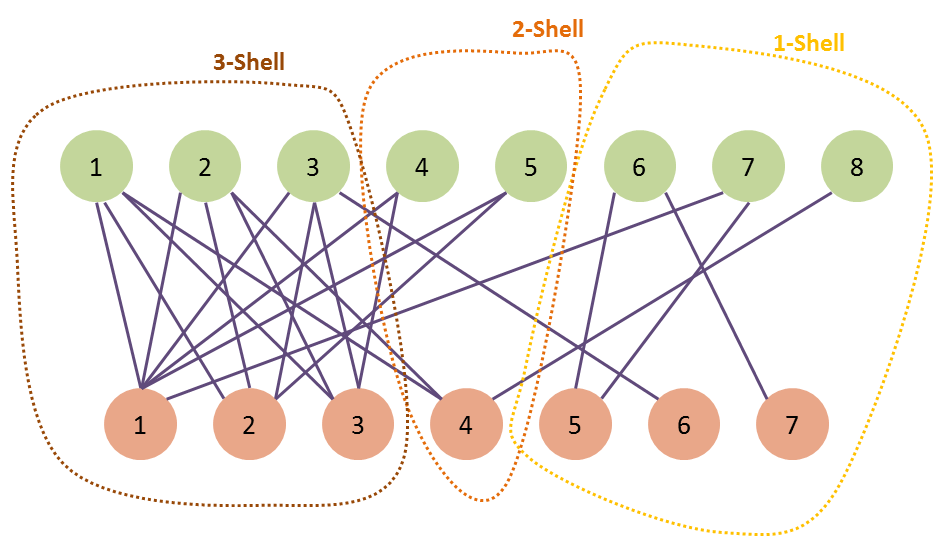
\includegraphics[scale=0.5]{Figures/ESTATICA_kcore_decomposition_example.png}
\caption{Descomposición \textit{k-core} de una red bipartita ficticia.}
\label{fig:ESTATICA_kcore_decomposition_example}
\end{figure}

Según la definición \ref{ESTATICA_def_kcore}, el  \textit{1-core} es la unión de las tres \textit{shell}, mientras que el \textit{2-core} es la unión de la \textit{2-shell} y la \textit{1-shell}. El \textit{k-core} máximo coincide con la  \textit{k-shell} máxima. 

Como estamos tratando de redes bipartitas, distinguimos dos subconjuntos en cada \textit{k-shell}, el de los nodos de la clase $A$ y el de los de la clase $B$. Los llamaremos $K^{A}_{j}, K^{B}_{j}$, donde  $j$ es el índice de la \textit{k-shell}.
Es posible que uno de ellos sea vacío, es decir, no todas las \textit{k-shell} tienen nodos de ambas clases necesariamente.
Al valor máximo de \textit{k}, lo llamamos $ks_{max}$, que corresponde a \textit{shell} más interna de la red $ks_{max}\equiv C^{A,B}$. Esta nomenclatura simplifica la definición de las \textit{k-magnitudes} que surgen de la red descompuesta siguiendo el procedimiento descrito, $C^A$ y $C^B$ son las especies de las \textit{shells} máximas de cada clase.


\section{Definición de las k-magnitudes}

Las especies más conectadas de una red mutualista son resistentes a las perturbaciones externas porque el beneficio que reciben depende de múltiples fuentes. Esta parece ser la razón por la que las redes mutualistas tienden al anidamiento, una conexión directa con el centro de la red aumenta las probabilidades de supervivencia. Para medir la 'distancia' desde un nodo cualquiera a la \textit{k-shell} más interna de la clase opuesta, hemos definido el \textit{$k_{radius}$}.

\begin{theo} 
El \textit{$k_{radius}$} de la especie $m$ de la clase $A$ es el valor medio de las distancias más cortas desde esta a cada una de las especies de $C^B$
\begin{align*}
\displaystyle
k^A_{radius}(m) = \frac{1}{\mid C^{B} \mid}\sum\limits_{j \in C^{B}} dist_{mj}  \qquad   m \in A
\stepcounter{equation}\tag{\theequation}\label{kradius}
\end{align*}
\label{ESTATICA_kradius}
\end{theo}

En la fórmula \ref{ESTATICA_kradius} $dist_{mj}$ es el camino más corto de la especie $m$ a cada una de las $j$ especies que forman el conjuto $C^B$. La misma definción es válida para especies de la clase $B$, calculando la distancia media a las especies de $C^A$. El valor mínimo posible de $k_{radius}$ es $1$ para un nodo perteciente a $C^B$ conectado con todas las especies de $C^A$ (y viceversa).

%\begin{figure}[h!]
%\centering
%\includegraphics[scale=0.58]{ESTATICA_red_example.eps}
%\caption {Cálculo de \textit{$k_{radius}$} y  \textit{$k_{degree}$} en una red ficticia.}
%\label{fig:ESTATICA_red_example}
%\end{figure}

\begin{figure}[h!]
\centering
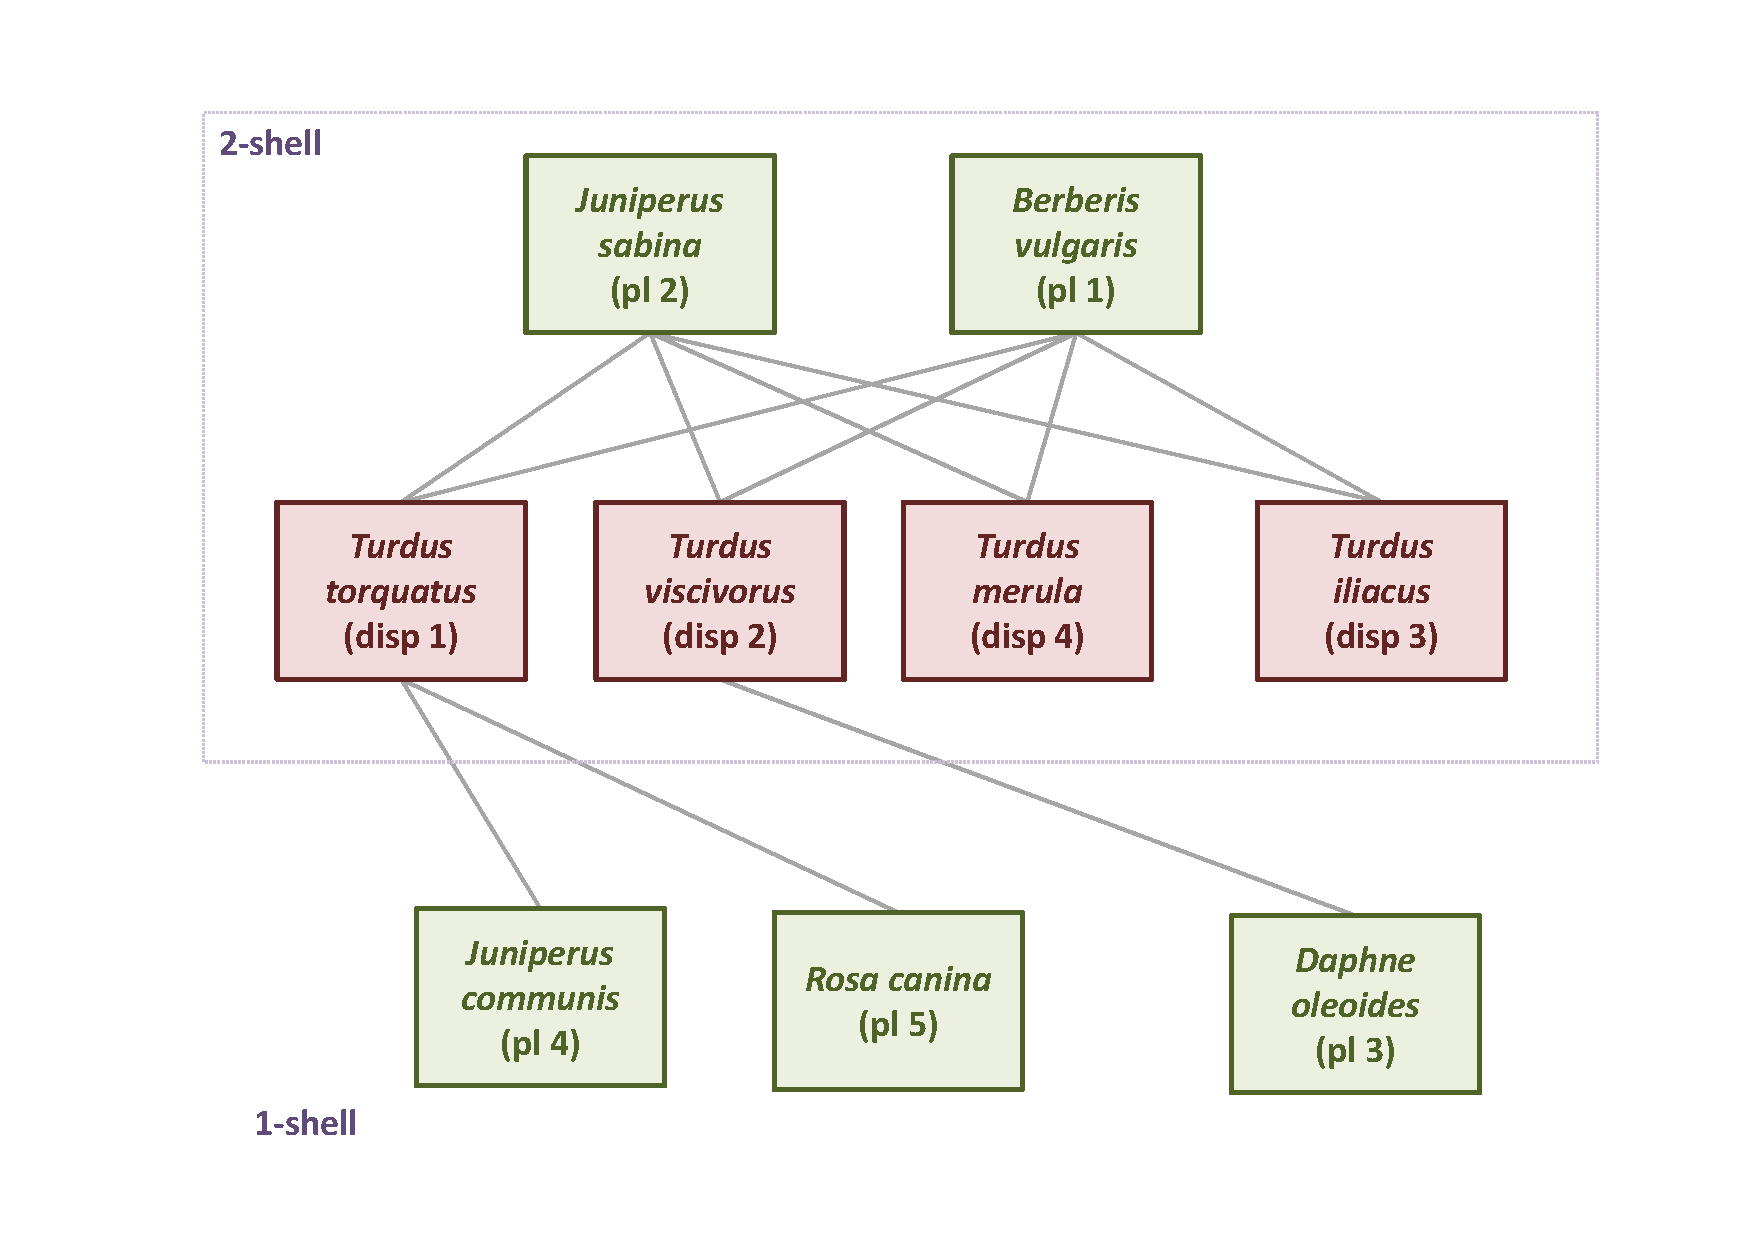
\includegraphics[scale=0.5]{Figures/ESTATICA_SD_030_example_network.pdf}
\caption {Red de frugívoros en Santa Bárbara, Sierra de Baza (España) \cite{jordano1993geographical}.}
\label{fig:ESTATICA_red_example}
\end{figure}

%La parte superior izquierda de la figura \ref{fig:ESTATICA_red_example} es el esquema de otra red ficticia muy sencilla, con solo siete nodos, tres de la clase $A$ y cuatro de la $B$. Como se puede ver,  la especie $B4$ es la única que pertenece a la $1$-$shell$. El resto son parte de las $2$-$shell$, que por ser la más internas se toman como referencia para medir los $k_{radius}$ individuales. 
%
%En la parte superior derecha de la imagen, se reproduce el detalle de las conexiones de la especie $A1$, perteneciente a $C^{A}$.  Como está directamente conectada con los tres nodos de $C^{B}$ la el camino más corto a cada uno de ellos es $1$, y en consecuencia $k^A_{radius}1$ es $1$. En la parte inferior derecha, la especie $A2$ que también pertenece a $C^{A}$ no tiene enlace directo con $B2$, aunque sí con $B1$ y $B3$. El camino más corto, marcado en color violeta, pasa por $B1$ y $A1$, y mide $3$. El $k^A_{radius}2$ vale $\sfrac{5}{3}$. En la parte inferior izquierda, vemos el esquema de conexiones de la especie $B4$, que no forma parte de $C^{B}$. Como cabía esperar, su$k_{radius}$ es mayor, $\sfrac{7}{3}$. 

La figura \ref{fig:ESTATICA_red_example} es una red de frugívoros real, de dimensiones muy reducidas, con cinco especies de plantas, cuatro de aves (mirlos) y once enlaces. Llamaremos clase $A$ a las plantas y clase $B$ a las aves. La descomposición \textit{k-core} se ha realizado con el algoritmo de \textit{pruning}. El índice $k$ máximo es $2$, todas las aves pertenecen a la \textit{2-shell}, no así todas las plantas. En este ejemplo todas las especies de la \textit{shell} máxima de la clase $A$ tienen enlace directo con todas las especies de la \textit{shell} máxima de la clase $B$, esto no tiene por qué ser siempre así. 

El camino más corto desde la planta $2$ a cada una de las cuatro especies de dispersores de la $2-shell$ es $1$ al estar enlazada con todas ellas. Su $k_{radius}$ es, en consecuencia, $1$ porque se ha definido como el promedio de las distancias a todas las especies de la \textit{shell} máxima de la clase contraria. Lo mismo ocurre con la planta $1$. Se puede comprobar que el $k_{radius}$ de todas las especies de aves de la $2$-$shell$ es también $1$, midiendo sus distancias respectivas a las plantas $1$ y $2$.

El cálculo es simple aunque algo más laborioso para las plantas de la $1$-$shell$. En la figura \ref{fig:ESTATICA_SD_030_example_distances} se ha tomado como ejemplo la especie número $4$. Hay que medir primero la distancia con cada una de las aves de la $2$-$shell$. Para ello, se han representado con distintos colores los caminos más cortos. La distancia con el dispersor $1$ es $1$ porque comparten enlace (camino en color azul marino). Con la especie $2$ no hay conexión directa, el camino más corto (representado en verde) es $pl4$-$disp1$-$pl2$-$disp2$ y la distancia es $3$. Lo mismo sucede con las especies de ave $3$ (camino rojo) y $4$ (camino violeta), ambas a distancia $3$ de la planta $4$. Medidas las cuatro distancias, ya se puede calcular el $k_{radius}$ de la especie de planta $4$, que es el promedio de 1, 3, 3 y 3, es decir 2,5. Este procedimiento hay que repetirlo para todas las especies de la red.

\begin{figure}[h!]
\centering
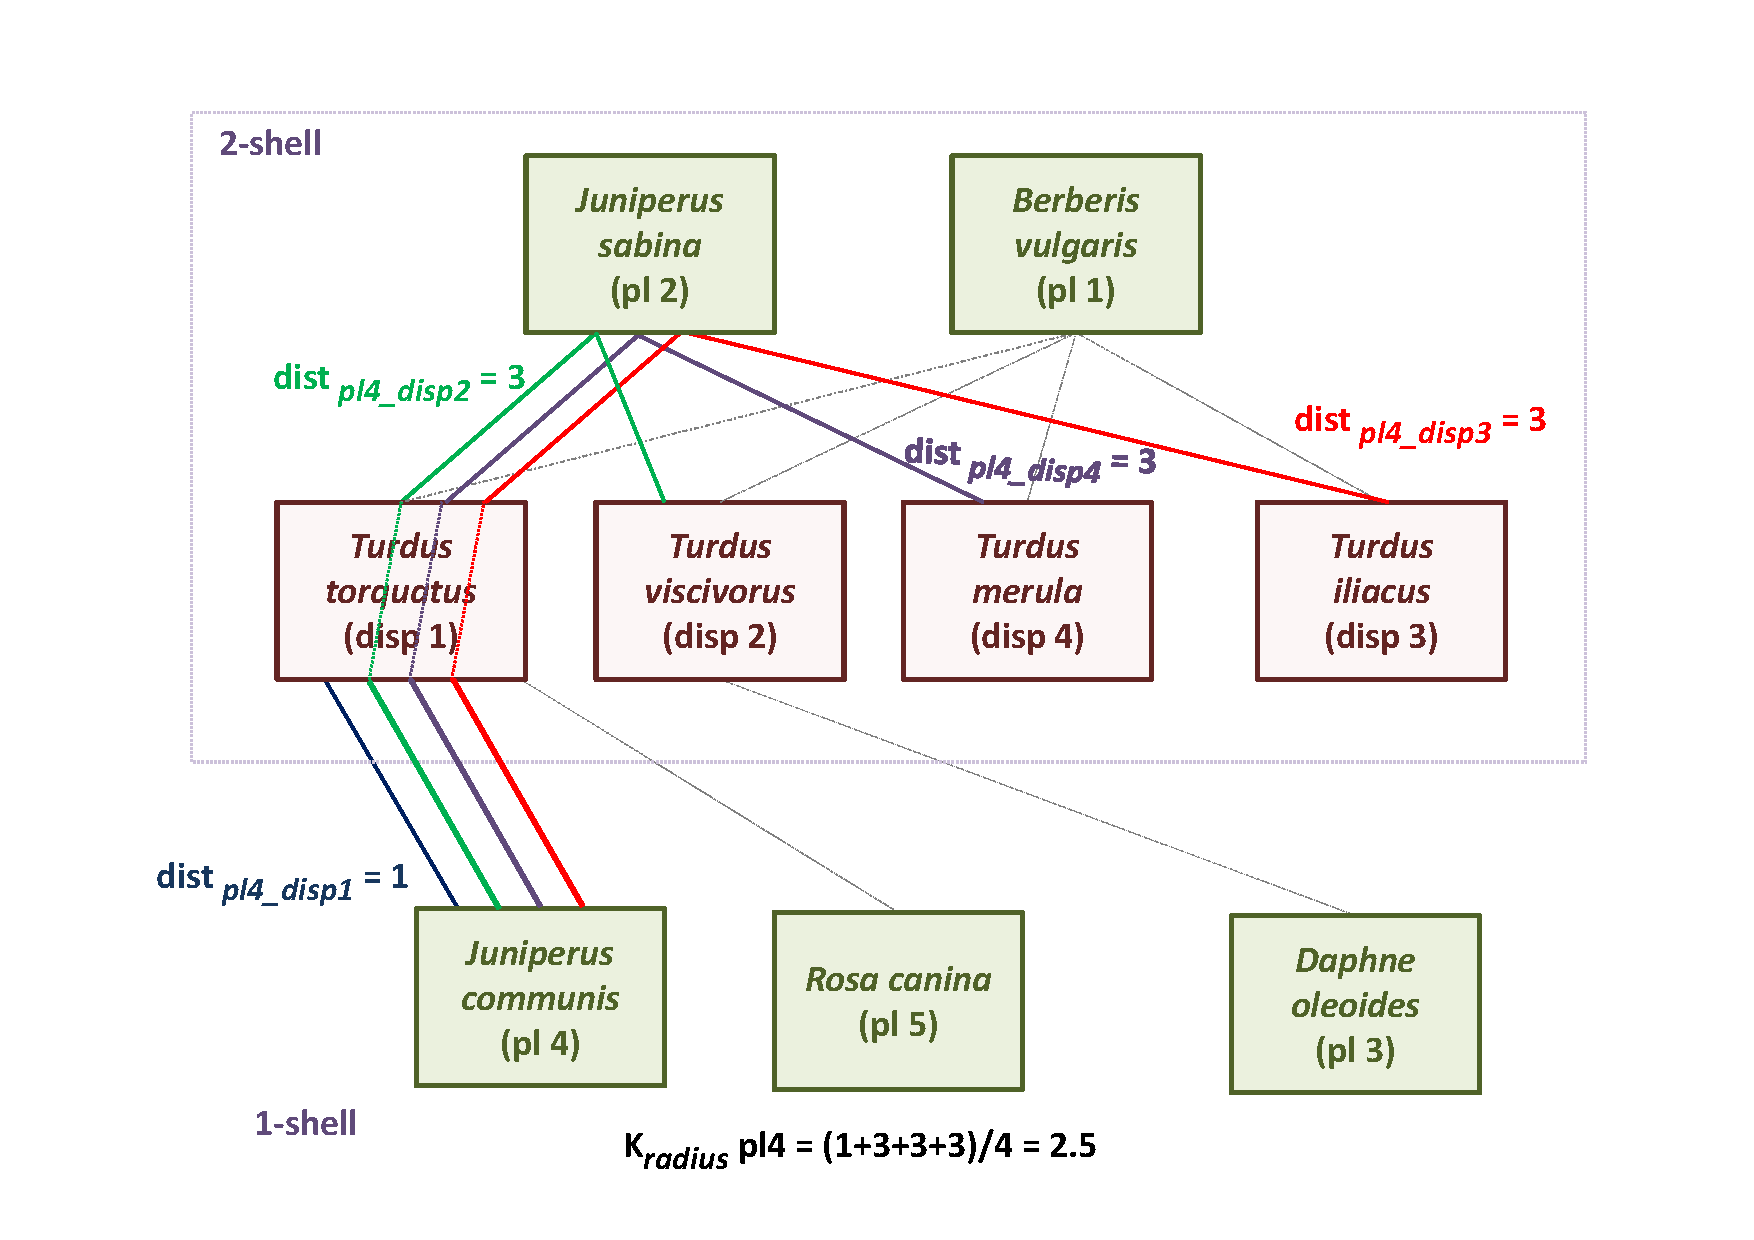
\includegraphics[scale=0.5]{Figures/ESTATICA_SD_030_example_distances.pdf}
\caption {Red de frugívoros en Santa Bárbara, Sierra de Baza (España) \cite{jordano1993geographical}.}
\label{fig:ESTATICA_SD_030_example_distances}
\end{figure}

Podemos definir una magnitud global, teniendo en cuenta los $k_{radius}$ de todas las especies.

\begin{theo} 
El \textit{$\overline k_{radius}$} de una red se obtiene promediando los ${k}_{radius}$ de todos los nodos, sin importar la clase a la que pertenezcan.
\begin{align*}
\displaystyle
\overline {k}_{radius} = \frac{1}{\mid A \cup B \mid}\sum\limits_{l \in A \cup B} k_{radius}\left(l\right)
\stepcounter{equation}\tag{\theequation}\label{avgkradius}
\end{align*}
\label{ESTATICA_avgkradius}
\end{theo}

Una red con todos sus nodos conectados (matriz de adyacencia cuadrada) tendría $\overline {k}_{radius}=1$, el menor posible. En una con matriz de adyacencia triangular el $\overline {k}_{radius}$ vale $1.5$. Intuitivamente, el $\overline {k}_{radius}$ será pequeño para redes muy anidadas, porque la probabilidad de conexión con la \textit{shell} más interna es elevada. Las especies generalistas están muy interconectadas y las especialistas tienen enlaces directos con las \textit{k-shells} de mayor índice. Por el contrario, una distribución de enlaces puramente aleatoria conduciría a una red con mayor $\overline {k}_{radius}$.

Es necesario aclarar en este punto que $\overline {k}_{radius}$ no es una medida de anidamiento, sino de compacidad. La noción de \textit{network compactness} se ha utilizado con diferentes sentidos y no siempre precisos en la literatura \cite{wagner2003does, egghe2003measure, chapanond2005graph, zhang2011constructing}. Nosotros utilizaremos una de las definiciones más laxas, la que indica que una red es compacta cuando los nodos se conectan de manera preferente a las partes más centrales \cite{alava2004preferential}. Es en este sentido en el que nos referiremos a $\overline {k}_{radius}$ como medida de compacidad de la red.

El ${k}_{radius}$ es una buena medida de conexión al corazón de la red pero no de centralidad. Por ejemplo, su valor es bajo para un especialista con un enlace a la \textit{shell} más interna, aunque sabemos que no resulta determinante para la estabilidad global de la red. Para atender esta necesidad, definimos una segunda \textit{k-magnitud}.

\begin{theo} 
El \textit{$k_{degree}$} de la especie $m$ de la clase $A$ es la suma de los inversos de los $k_{radius}$ de las especies de la clase $B$ que tienen enlace directo con ella.
\begin{align*}
\displaystyle
k^A_{degree}(m) = \sum\limits_{j} \frac{a_{mj} }{k^B_{radius}\left(j\right)}  \quad   m \in A, \forall j \in B
\stepcounter{equation}\tag{\theequation}
\end{align*}
\label{kdegree}
\end{theo}

Donde $a_{mj}$ es el elemento de la matriz de interacción que representa el enlace, cuyo valor es $1$ si existe o $0$ si no está presente. El $k_{degree}$ es la suma de los inversos de los $k_{radius}$ de los nodos conectados con $m$. Una especie de la \textit{shell} más interna tiene un $k_{degree}$ elevado,  mientras que los especialistas con solo uno o dos enlaces tiene un $k_{degree}$ reducido. 

En el ejemplo de la figura \ref{fig:ESTATICA_red_example}, vamos a calcular el $k_{degree}$ de la planta $1$. Se obtuvo que el $k_{radius}$ de las cuatro especies de la $2$-$shell$ de dispersores es $1$. Al tener la planta enlace con cada una de ellas, el $k_{degree}$, que es la suma de los inversos de los $4$ valores de $k_{radius}$, vale $4$. Si ahora nos fijamos en la planta $4$, solo tiene un enlace con el dispersor $1$, cuyo $k_{radius}$ es $1$ y así el $k_{degree}$ de la planta $1$ vale solo $1$. De manera intuitiva, la planta $1$ parece ser menos importante para la supervivencia de la red que la planta $4$. 

Por último, vamos a calcular el $k_{degree}$ de la especie de pájaro $1$:
\begin{equation}
k^B_{degree}\left(1\right) = \frac{1}{k^A_{radius}\left(1\right)} + \frac{1}{k^A_{radius}\left(2\right)} + \frac{1}{k^A_{radius}\left(4\right)} + \frac{1}{k^A_{radius}\left(5\right)} = 2,8
\label{example_kdegree}
\end{equation}

Al igual que se ha definido el $\overline k_{radius}$ podemos definir el grado medio de una red:
\begin{theo} 
El \textit{$\overline k_{degree}$} de una red se obtiene promediando los ${k}_{degree}$ de todos los nodos, sin importar la clase a la que pertenezcan.
\begin{align*}
\displaystyle
\overline {k}_{degree} = \frac{1}{\mid A \cup B \mid}\sum\limits_{l \in A \cup B} k_{degree}\left(l\right)
\stepcounter{equation}\tag{\theequation}\label{avgkdegree}
\end{align*}
\label{ESTATICA_avgkdegree}
\end{theo}

El  $\overline k_{degree}$ recuerda el \textit{índice de Harary} que se deine como la suma de los inversos de las distancias entre todos los nodos de un grafo conectado \cite{plavvsic1993harary}. El  $\overline k_{degree}$ solo tiene en cuenta los enlaces con la \textit{shell} máxima y utiliza el inverso de los $k_{radius}$, no de las distancias.

En la tabla \ref{table:table_SD_030} pueden consultarse los valores de las \textit{k-magnitudes} de la red que se ha utilizado como ejemplo.

\begin{table}[htbp]
\small
  \centering
    \begin{tabular}{rrr}
    \toprule
    $Especie$ & $k_{radius}$ & $k_{degree}$  \\
    \midrule
    pl1  & 1    & 4 \\
    pl2  & 1    & 4 \\
    pl3  & 2,5  & 1 \\
    pl4  & 2,5  & 1 \\
    pl5  & 2,5  & 1 \\
    disp1 & 1    & 2,8 \\
    disp2 & 1    & 2,4 \\
    disp3 & 1    & 2 \\
    disp4 & 1    & 2 \\
    \bottomrule
    \end{tabular}%
  \caption{\label{table:table_SD_030} \textit{K-magnitudes} de la red de la figura \ref{fig:ESTATICA_SD_030_example_distances}. Valores globlales: $\overline k_{radius} = 1,5 $ y $\overline k_{degree} = 2,24$.}
\end{table}%

\section{Material y métodos}

Para este capítulo hemos utilizado la colección de datos de redes mutualistas de la \textit{Web of Life}  \url{http://www.web-of-life.es/} \cite{fortuna2014web}. Hemos analizado todas las disponibles en las categorías \textit{planta-polinizador} y \textit{planta-dispersor de semillas}. En diciembre de 2015 dicha colección consta de 59 redes de la primera familia y 30 de la segunda. El número de especies por red varía entre 6 y 997 y el número de interacciones entre 6 y 2993.

El software se ha desarrollado en \texttt{R} y \texttt{Python}. La \textit{descomposición k-core} se realiza con el paquete \texttt{R} \texttt{igraph} \cite{csardi2006igraph}. El mismo paquete ofrece funciones para el cálculo de $NODF$ y $Modularity$. El código \texttt{R} para medir ${k}_{degree}$ y ${k}_{radius}$ es propio. Los valores medios de estas magnitudes se calculan descartando las especies que no pertenecen a la componente gigante cuando en la red se produce esta circunstancia. 

\subsection{Análisis mediante modelo nulo}
\label{sec:nullmodels}

El análisis de modelo nulo es una técnica para evaluar la significación estadística de las magnitudes de red y resulta imprescindible cuando estas no son libres de escala \cite{gotelli1996null}. En particular se ha aplicado en diversos trabajos para estudiar la validez de las distintas medidas de anidamiento \cite{ulrich2013pattern, feng2014heterogeneity} y modularidad \cite{fortuna2010nestedness, mello2011modularity}. En esta investigación se emplea para comparar el comportamiento de $\overline k_{radius}$ y de la medida de anidamiento $NODF$.

Un modelo nulo no es más que una modificación aleatoria de la red original. Para valorar la significación estadística de un índice, se genera un
número elevado de redes según el modelo nulo y se construye la distribución de probabilidad, que tenderá, por el teorema del límite central, a una gaussiana. Si el valor de la red real no se debe a puro azar sino a una propiedad intrínseca, será significativo desde el punto de vista estadístico. De forma habitual se considera que esto es así
si se aleja al menos dos desviaciones estándar de la media estimada. En general se utilizarán unidades reducidas en este procedimiento \textit{z scores}.

Hay numerosos modelos nulos disponibles, en función de los criterios con que se desee construir la red modificada. Esto plantea un reto a los investigadores porque los resultados y las conclusiones que se desprendan de ellos dependerán del modelo elegido \cite{ulrich2007null,gotelli2012statistical}. Así, si se utilizan modelos muy restrictivos, no puede afirmarse que las redes mutualistas sean fuertemente anidadas, en especial las que tienen matriz de interacción pesada \cite{joppa2010nestedness, staniczenko2013ghost}. Si se utilizan modelos menos condicionados, el anidamiento es entonces más habitual, como indicaba el trabajo seminal de Bascopmte \textit{et al} \cite{bascompte2003nested}.

En este estudio se han utilizado los dos modelos nulos de uso más frecuente en el análisis de redes binarias y pesadas, ambos disponibles como funciones del paquete \texttt{bipartite} en lenguaje \texttt{R} \cite{dormann2008introducing}. Para las pesadas, se emplea el modelo \texttt{swap.web}, en el que se conservan la conectancia y las distribuciones marginales \cite{ dormann2009indices}. Para las redes binarias se ha escogido el modelo \texttt{mgen} que devuelve un modelo aleatorio que conserva tan solo el número de enlaces de la red original \cite{vazquez2009evaluating}. Este segundo es mucho menos restrictivo que el primero.

\begin{figure}[hp!]
\centering
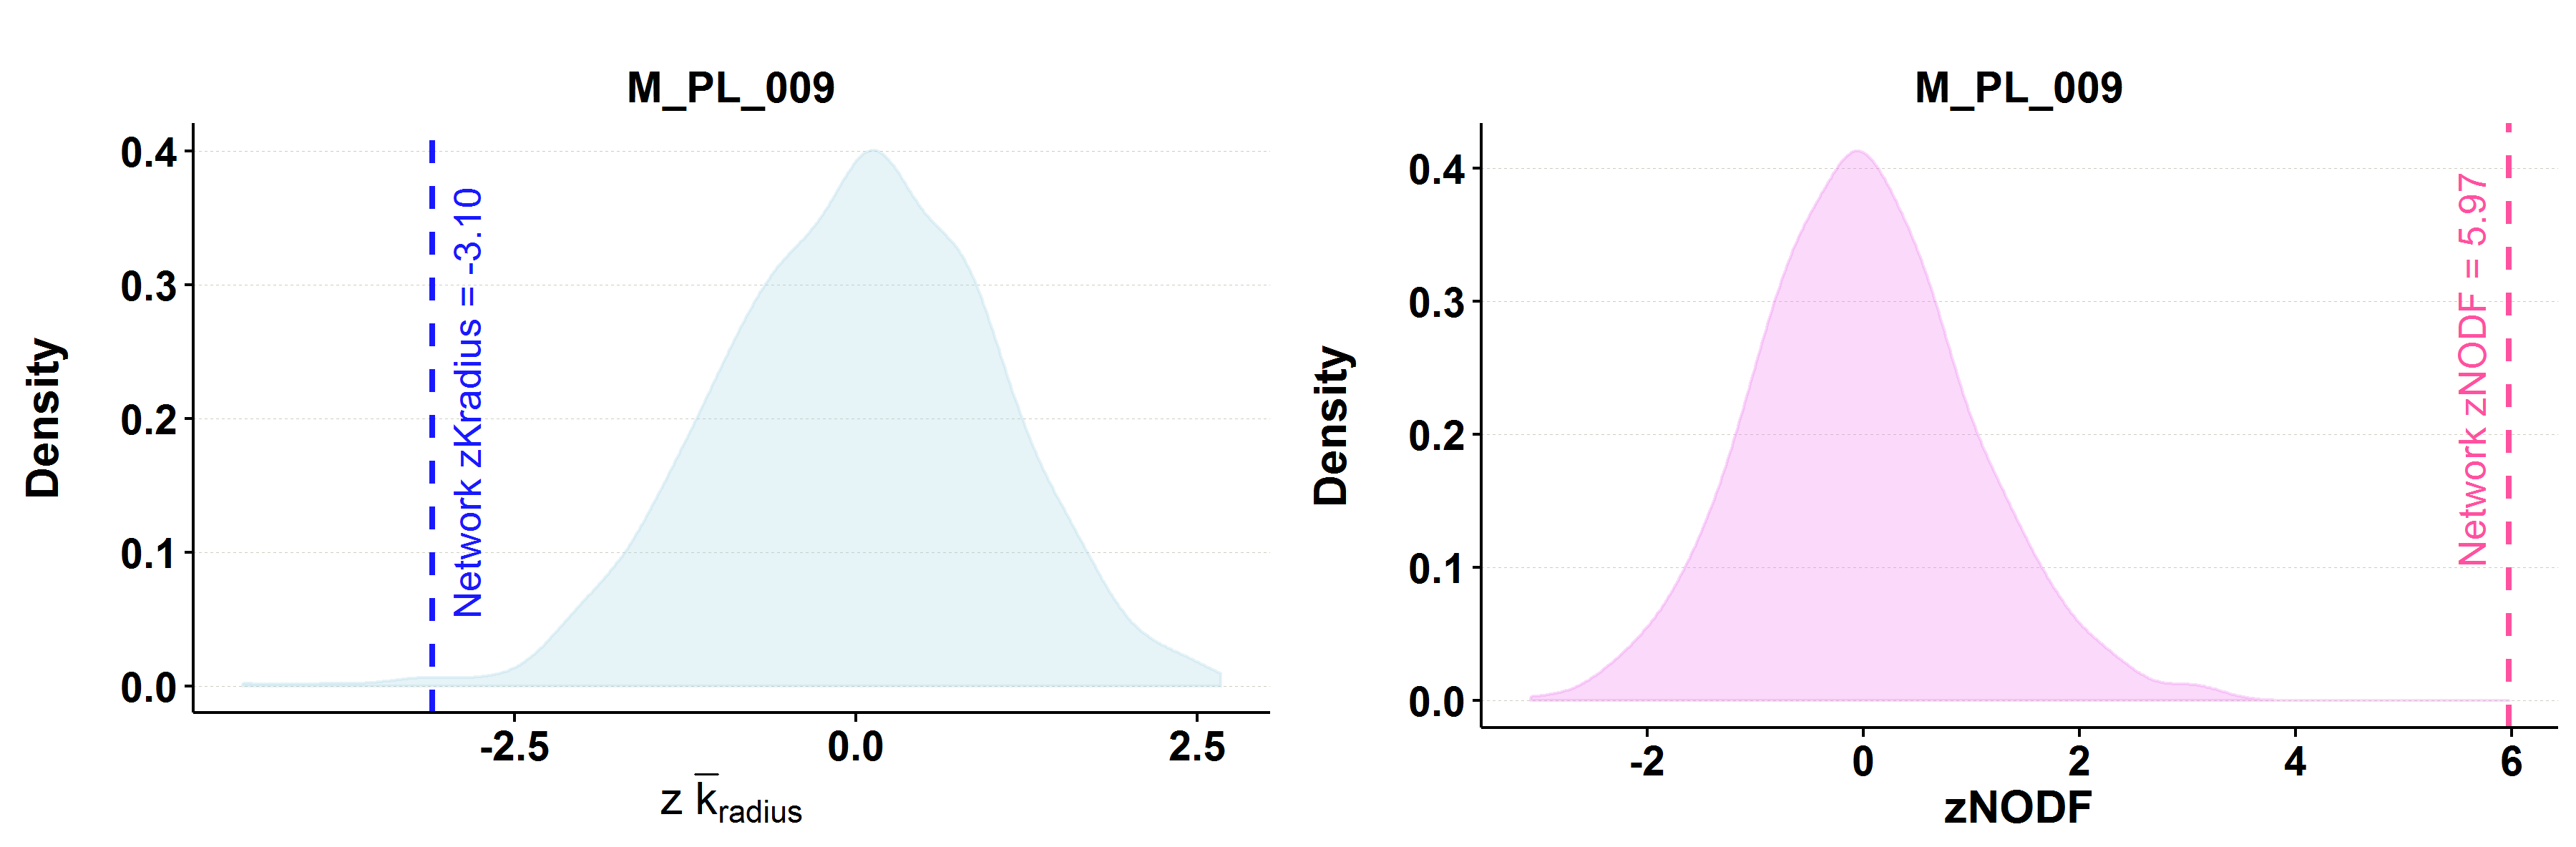
\includegraphics[scale=0.5]{Figures/ESTATICA_zALL.png}
\caption{Ejemplo de $z scores$ de $NODF$ y $z\overline k_{radius}$ para una red de polinizadores con matriz de interacción binaria \cite{elberling1999structure} }
\label{fig:ESTATICA_zALL}
\end{figure}

El propósito no es llevar a cabo un análisis exhaustivo con modelos de diferente nivel de restricción sino comparar el comportamiento de $\overline k_{radius}$ con el de $NODF$. Para
cada red se generan $1000$ modelos nulos con los que se construyen las distribuciones de probabilidad de $NODF$ y $\overline k_{radius}$. El valor $zNODF$ de la red original es estadísticamente significativo si es mayor que $2$, ya que este índice crece con el anidamiento, en tanto que $z\overline k_{radius}$ debe ser menor que $-2$ para que se pueda afirmar que la red es compacta (figura \ref{fig:ESTATICA_zALL}).

\subsection{Experimento de recableado}

El objetivo de este experimento es comparar la alteración de $NODF$ y $\overline k_{radius}$, para una red dada, cuando algunos de sus enlaces se recablean de forma aleatoria. Para ello se mide la correlación de ambas magnitudes. Este procedimiento se aplica solo a las redes binarias, por la complejidad de definir un método de recableado para las pesadas que no altere por completo su estructura.

Se empieza cambiando el uno por ciento de los enlaces, seleccionados al azar sin reemplazo. Las \textit{k-magnitudes} de la red alterada se calculan y se almacenan. La operación se repite con el porcentaje ente $1$ y $50$ en $25$ pasos. El recableado se aplica siempre a la red original, no es acumulativo. 

El experimento se repite $10$ veces para cada red. Es equivalente a un modelo nulo que conserva el número de enlaces pero en el que solo se deja espacio al azar en un porcentaje reducido. La evolución de $NODF$ y $\overline k_{radius}$ y de sus \textit{z scores} puede así compararse con los parámetros de la red original y con los del modelo nulo explicado en la sección \ref{sec:nullmodels} (figura \ref{fig:z_M_PL_012_rewire_Binary_ES_model_5}).

\begin{figure}[h!]
\centering
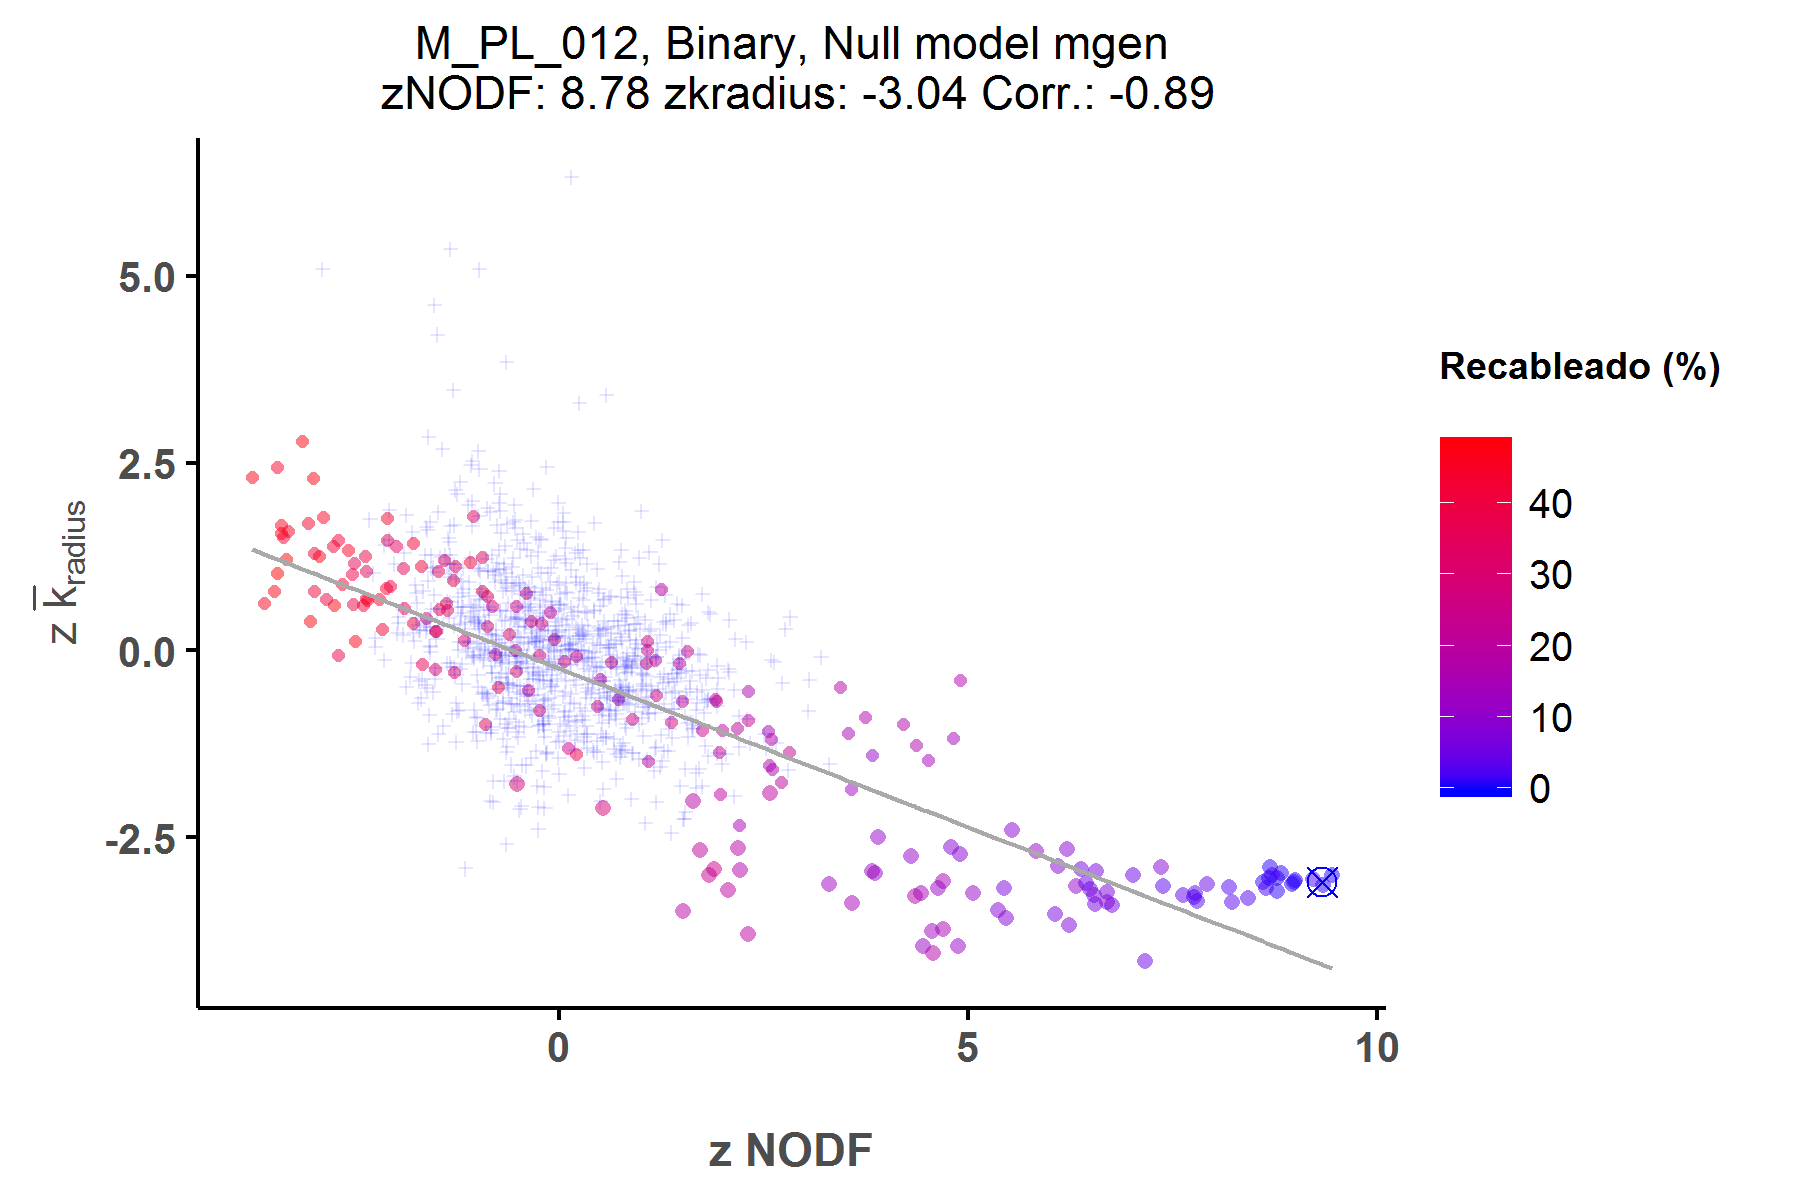
\includegraphics[scale=0.75]{Figures/ESTATICA_z_M_PL_012_rewire_Binary_ES_model_5.png}
\caption {Gráfica del experimento de recableado para la red de polinizadores número $12$ (Parque de Garajonay, compilada por Olesen, no publicada). La nube de cruces pequeñas representa los pares de valores $zNODF,z\overline k_{radius}$ de las $1000$ realizaciones del modelo nulo. Los puntos representan ese par de valores para cada red recableada. El aspa azul dentro de un círculo señala los valores de $zNODF,z\overline k_{radius}$ de la red original. En gris, el resultado de la regresión lineal para los valores de las redes recableadas.}
\label{fig:z_M_PL_012_rewire_Binary_ES_model_5}
\end{figure}

\clearpage
\section{Resultados}

En este apartado se describen los resultados de los siguientes procedimientos: análisis exploratorio de los datos de las redes de la colección, estudio de la correlación entre las \textit{k-magnitudes} las medidas estadísticas habituales, análisis mediante modelo nulo y experimento de recableado.

\subsection{Análisis exploratorio}

La figura \ref{fig:ESTATICA_hist_kmagnitudes} contiene los histogramas de las tres \textit{k-magnitudes} globales que describen las redes incluidas en la investigación. En la mitad de ellas el $k$ máximo es $4$ o inferior y solo hay dos en las que este índice supere $8$. La distribución del $\overline{k}_{radius}$ es aproximadamente normal, con una mediana de $2,51$ y media $2,47$. Teniendo en cuenta que el valor mínimo de esta magnitud es $1$, podemos deducir que las redes mutualistas analizadas son \textit{very small world}, las especies se encuentran muy próximas a la \textit{k-shell} más interna. Este dato concuerda con la observación de que los especialistas se conectan con generalistas lo que les proporciona más probabilidades de supervivencia. Finalmente, el $\overline{k}_{degree}$ se
concentra entre los valores $0,5$ y $3,5$ con la mediana en $2,08$. La conectividad media de las redes es reducida
porque abundan los especialistas. En el tercer histograma hay una diferencia sensible entre las redes de polinizadores
y las de dispersores de semillas, estas últimas tienen valores más elevados.

\begin{figure}[h!]
\centering
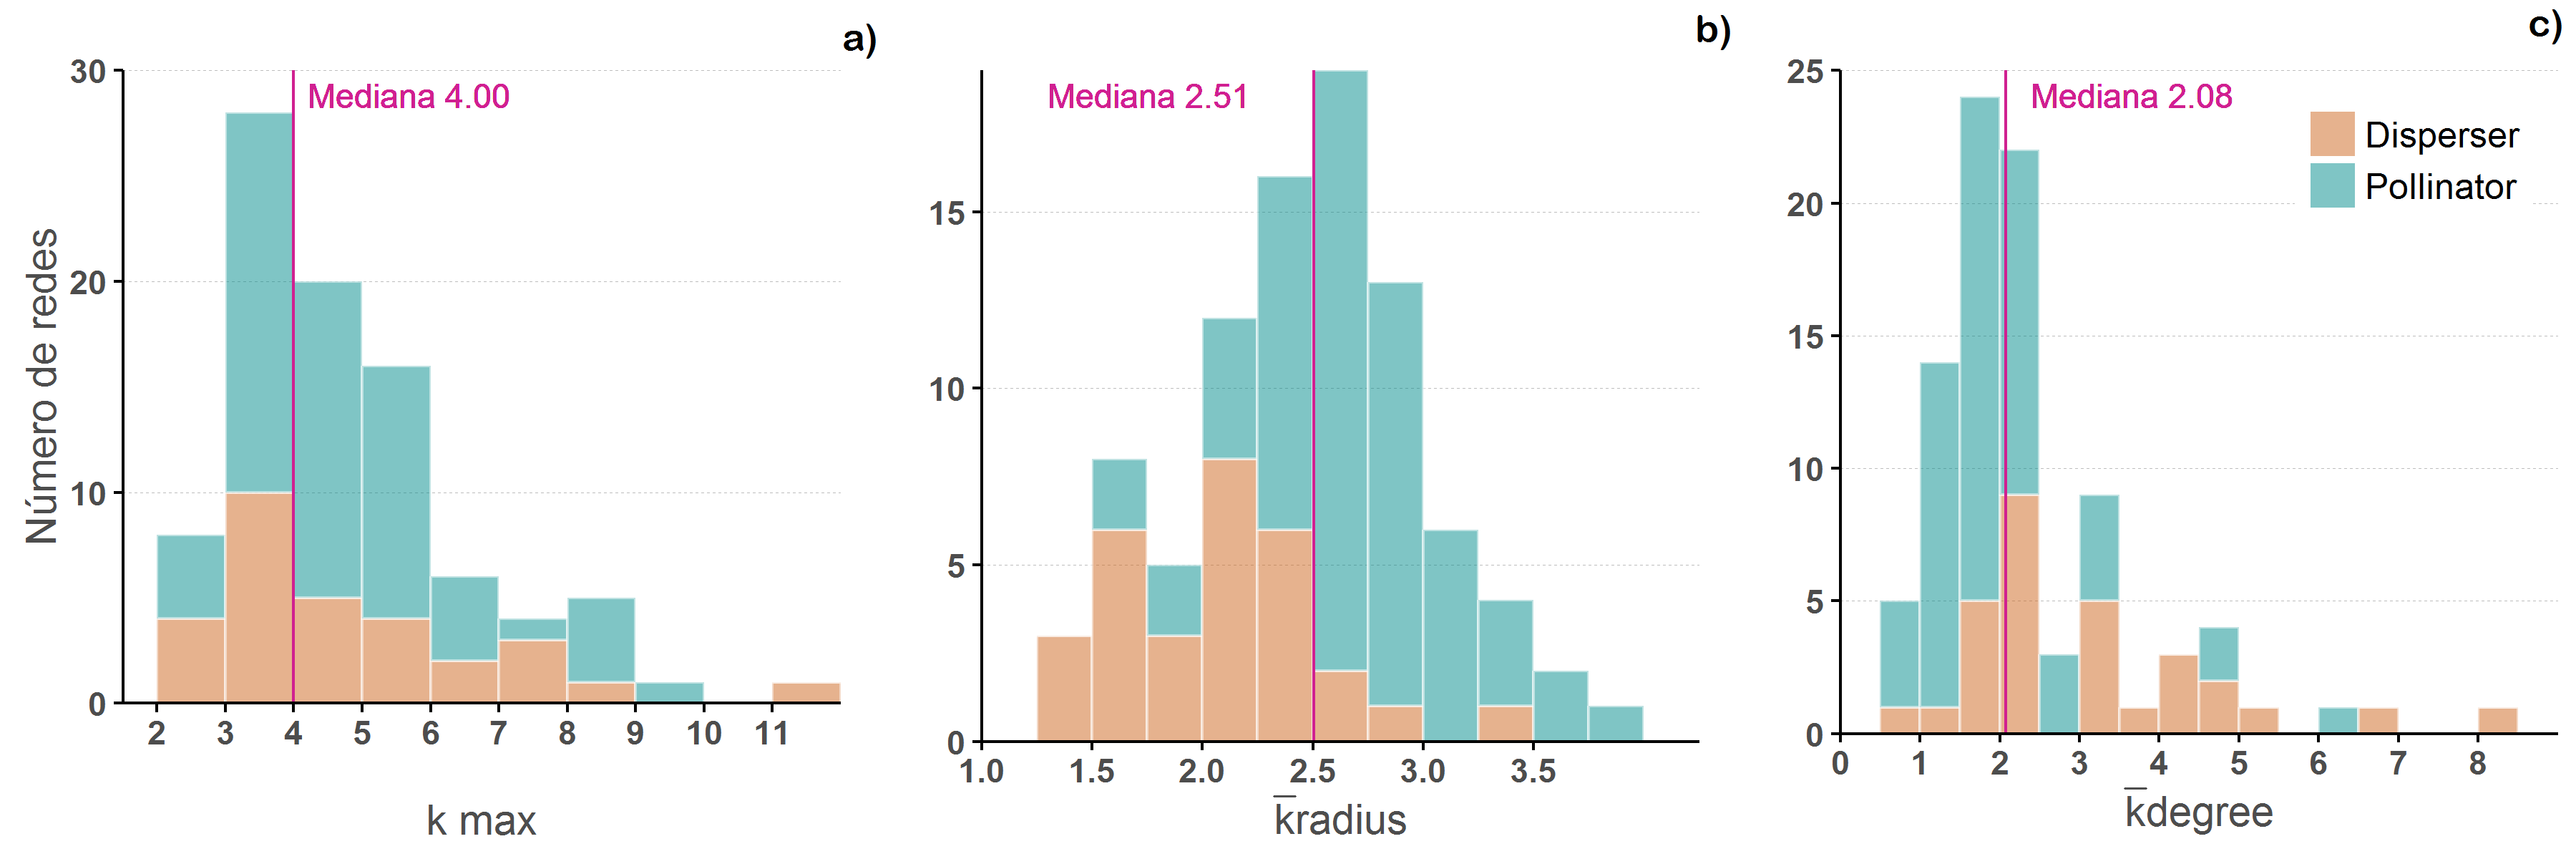
\includegraphics[scale=0.5]{Figures/ESTATICA_hist_kmagnitudes.png}
\caption{Histogramas de las \textit{k-magnitudes}.}
\label{fig:ESTATICA_hist_kmagnitudes}
\end{figure}

En una primera aproximación visual a los datos, se observa que que existe una correlación notable entre el $\overline{k}_{radius}$ de la red y el número de especies (figura \ref{fig:ESTATICA_tamanyo_kdegree_kradius}), impresión que confirman los datos de la regresión lineal. Como cabía esperar, cuanto mayor es la red, mayor es la distancia media a la \textit{shell} máxima. El crecimiento sigue una ley logarítmica, nótese la escala del eje $X$. Sucede algo parecido con el número de enlaces, pero en este caso se puede apreciar mayor dispersión. Podemos concluis que $\overline{k}_{radius}$ no es libre de escala.

Por el contrario, $\overline{k}_{degree}$ no parece guardar relación con el tamaño de la red, ya se mida en número total de especies o de enlaces. Para la mayoría de redes su valor está en torno a $2$. Este dato hace sospechar que la distribución de ${k}_{degree}$ en las redes es muy heterogénea. La mayoría de los nodos tienen valores bajos, por lo que la media arroja ese valor tan reducido. En la figura \ref{fig:ESTATICA_density_plots} aparecen las gráficas de dicha distribución en tres redes en las que resulta evidente la asimetría. 

\begin{figure}[h!]
\centering
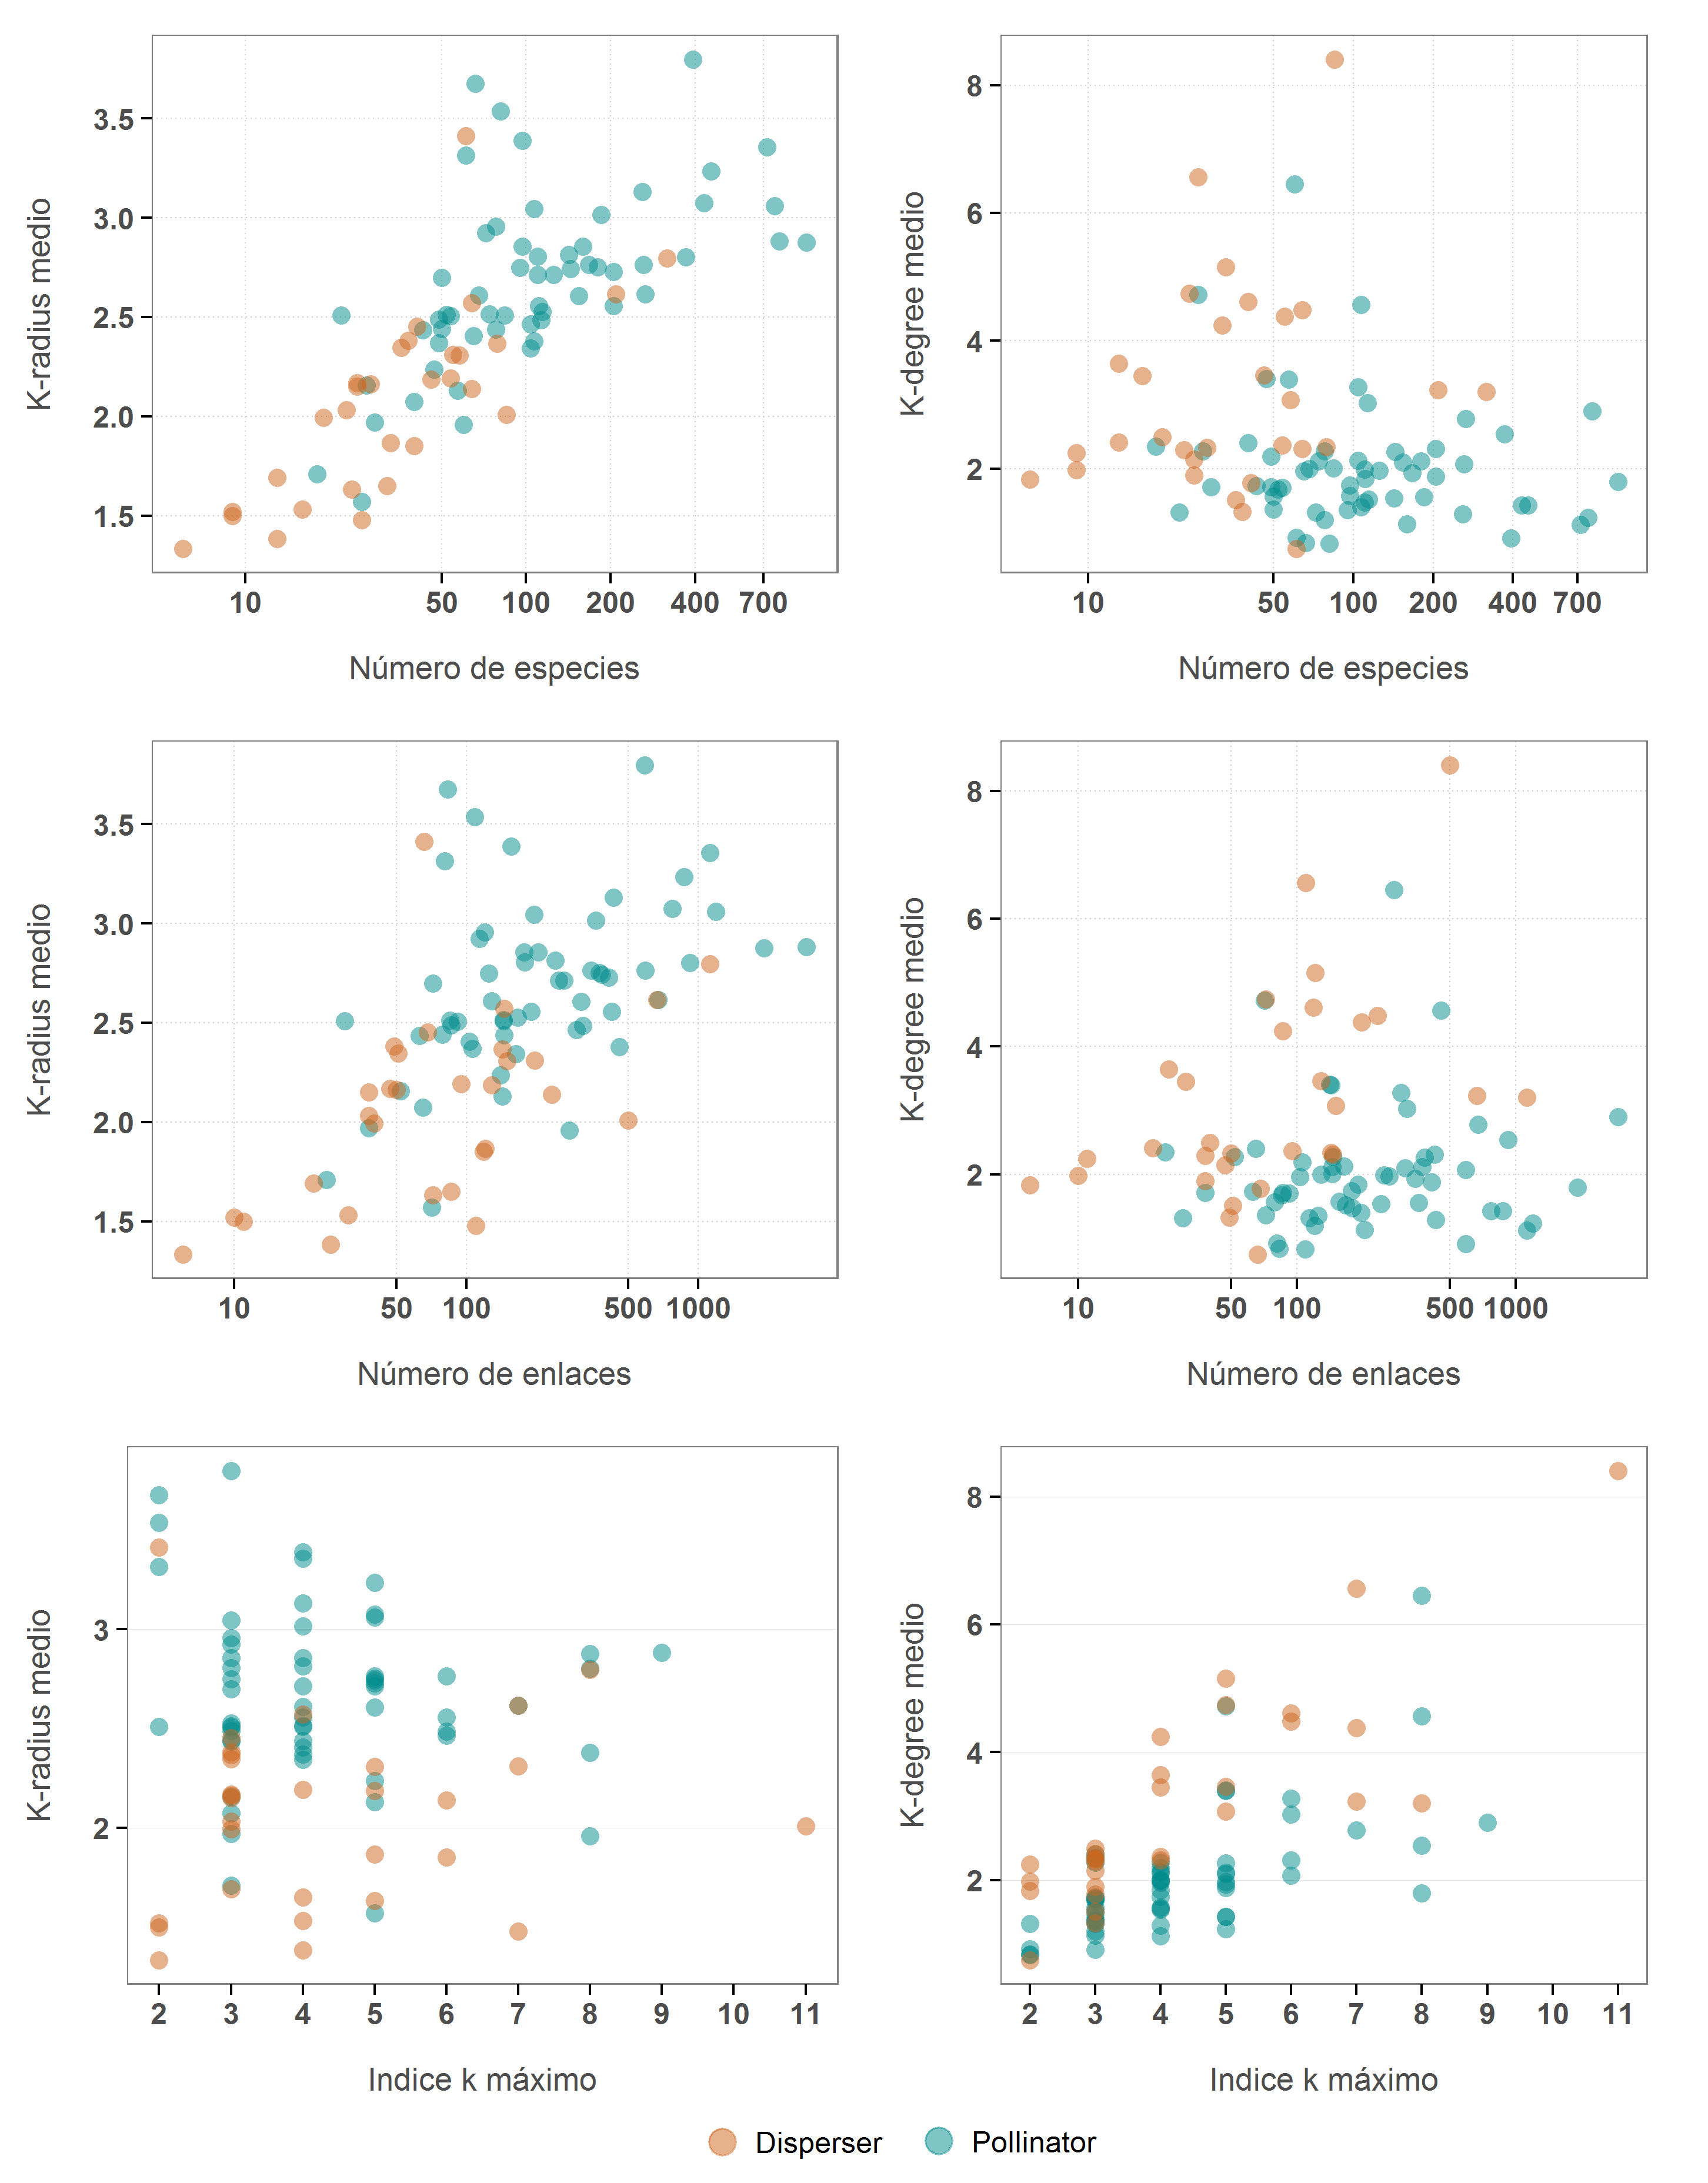
\includegraphics[scale=0.55]{Figures/ESTATICA_tamanyo_kdegree_kradius.png}
\caption{Diagramas de dispersión que relacionan las \textit{k-magnitudes} con el tamaño de la red.}
\label{fig:ESTATICA_tamanyo_kdegree_kradius}
\end{figure}

Al observar la relación entre las dos \textit{k-magnitudes} y el índice $k$ máximo de la red, se descubre que el comportamiento es diferente. El $\overline{k}_{radius}$ no guarda relación con el $k$ máximo y se observa una importante dispersión de valores para un mismo índice $k$ máximo. Este dato puede resultar paradójico pues un $k$ elevado significa que en la red puede haber caminos largos. No obstante, el cálculo de $\overline{k}_{radius}$ se hace con los caminos más cortos, y al existir una alta conectividad directa con la \textit{shell} más interna, este no es el factor más determinante. La correlación de $\overline{k}_{degree}$ crece con el $k$ máximo es notable. El $k$ máximo crece con la conectividad, y en consecuencia es lógico que $\overline{k}_{degree}$ se comporte de forma similar a este índice.

\subsection{Relación entre las medidas de grado}

La distribución de grado de las redes mutualistas sigue una ley de potencia truncada \cite{jordano2003invariant,vazquez2005degree}. El grado se utiliza de manera habitual en el análisis de redes como indicador de importancia del nodo. Se mide con facilidad pero no está exento de inconvenientes. Por ejemplo, dos especies de una red mutualista con el mismo grado pueden pertenecer a \textit{k shells} diferentes, o incluso siendo de la misma, estar conectados con nodos de $k_{radius}$ dispares.

La descomposición \textit{k core} ha permitido definir el $k_{degree}$ como un grado ponderado por la la inversa del $k_{radius}$ de las especies conectadas. 

Los dos índices guardan una correlación muy elevada para todas las redes, como se aprecia en el histograma de la figura \ref{fig:ESTATICA_ALL_plots_kdegree_degree_M_PL_001_ES}. A su derecha se ha representado el diagrama de dispersión para una red concreta, la relación cuasi lineal es similar para el resto. Los valores de la recta de regresión indican que para este caso, $k_{degree}$ se puede predecir de forma muy aproximada, multiplicando por $0.4$ el grado de la especie. La constante multiplicativa es siempre inferior a la unidad, porque la aportación a $k_{degree}$ de cada enlace se divide por el $k{radius}$ de la especie conectada que, por definición, es mayor o igual que $1$. 

Cabe preguntarse para qué crear un índice que no es más que otro ya existente multiplicado por una constante. La razón se entenderá observando con atención los diagramas de la fila inferior. El de la izquierda es la distribución de grado de la red, con su forma característica de ley de potencia truncada. En el del centro, se representa la función de distribución de $k_{degree}$. La escala de los ejes $X$ no es la misma, porque el rango de $k_{degree}$ es inferior como se acaba de explicar, pero empleando la misma anchura de diagrama es fácil ver que las figuras son muy parecidas.

En la última gráfica, se realiza una transformación simple. Los valores de $k_{degree}$ se dividen por el coeficiente $\alpha$ de la correlación lineal y el resultado (en turquesa) se superpone a la distribución de grado (en verde). Con esta representación queda claro que $k_{degree}$ no es un meramente el grado escalado. Lo que hace es transformar la distribución discreta de grado en otra con muchos más puntos intermedios, con lo que se obtiene una ordenación con criterio topológico de los nodos de idéntico grado. Esta sutil diferencia es importante a la hora decidir qué nodos son más importantes para la supervivencia de la red. La utilidad de este índice frente al grado se describe con detalles numéricos en el capítulo \ref{ChapterDESTRCCION}.

\begin{figure}[h!]
\centering
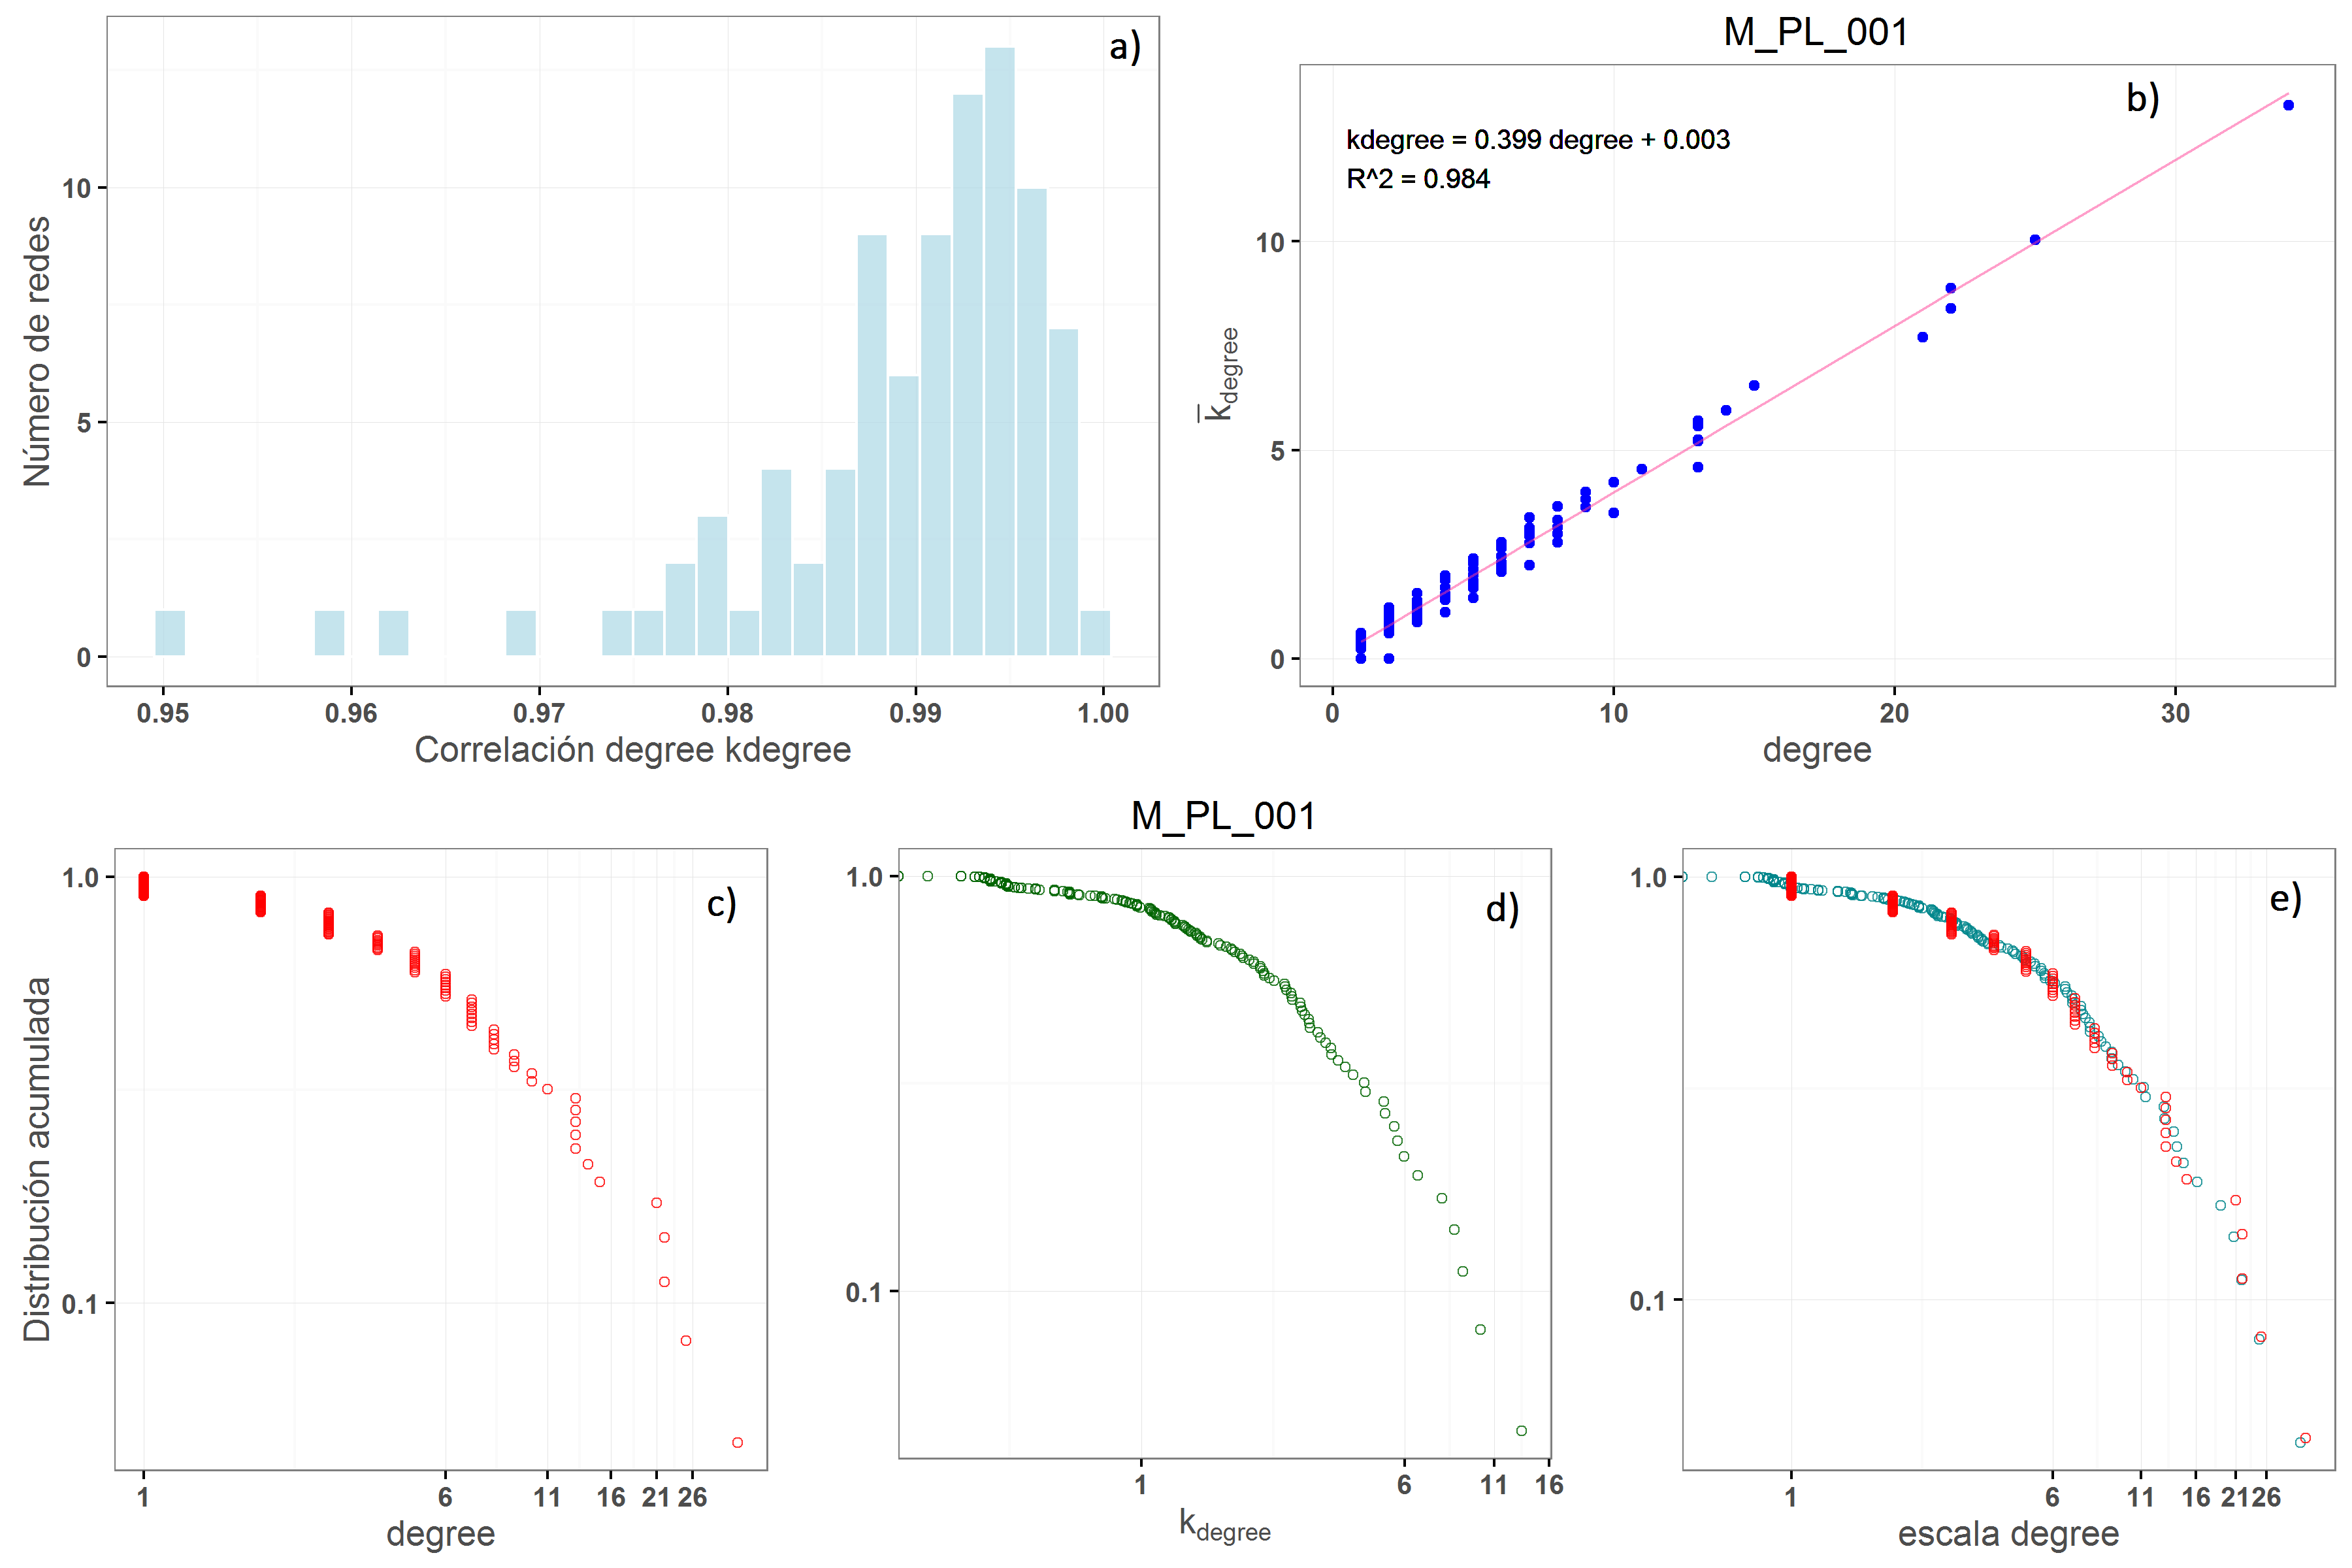
\includegraphics[scale=0.5]{Figures/ESTATICA_ALL_plots_kdegree_degree_M_PL_001_ES.png}
\caption{Relación entre $degree$ y $k_{degree}$. Arriba a la izquierda, histograma de la correlación entre ambas magnitudes para todas las redes del estudio. A su derecha, diagrama de dispersión de ambas magnitudes para la red de polinizadores $001$ y valores de la regresión lineal para esta red. En la fila inferior, funciones de distribución de los dos índices. En el tercer diagrama se han representado ambos, sobre la escala de $degree$ con la transformación en el eje $X$ $k_{degree} = \alpha * degree$ siendo $\alpha$ el coeficiente de regresión lineal que en este caso vale aproximadamente $0.4$.}
\label{fig:ESTATICA_ALL_plots_kdegree_degree_M_PL_001_ES}
\end{figure}


\subsection{Correlación entre \textit{k-magnitudes} y propiedades globales}
\label{subsection:Correlacion}

Uno de los objetivos principales de la investigación es hallar la posible relación entre las magnitudes que se derivan de la \textit{descomposición k-core} y las que se utilizan habitualmente en la caracterización del mutualismo. Hemos encontrado que las \textit{k-magnitudes} globales tienen una fuerte correlación con estas dos medidas, y esto es de gran interés puesto que surgen de la agregación de las propiedades locales de cada nodo.

Para realizar la comparación se calcula el anidamiento mediante \textit{NODF} y la modularidad siguiendo los procedimientos de cálculo descritos en el apartado \ref{sec:prop_mutualismo} \footnote{Para evitar confusiones entre el nombre la de la magnitud y la medida según un algoritmo concreto, en lo sucesivo se emplea \textit{Modularity}, en inglés y con mayúscula.}. Ambas medidas pueden obtenerse con el paquete \texttt{bipartite} en \texttt{R}. En la figura \ref{fig:ESTATICA_corrfigs} se han representado el $\overline {k}_{radius}$ en función de $NODF$ y el $\overline {k}_{degree}$ en función de la $modularidad$. Las figuras sugerían que existe un fuerte correlación negativa entre el $\overline {k}_{radius}$ y $NODF$ por una parte y, por otra, entre el $\overline {k}_{degree}$ y la $modularidad$. 

\begin{figure}[h!]
\centering
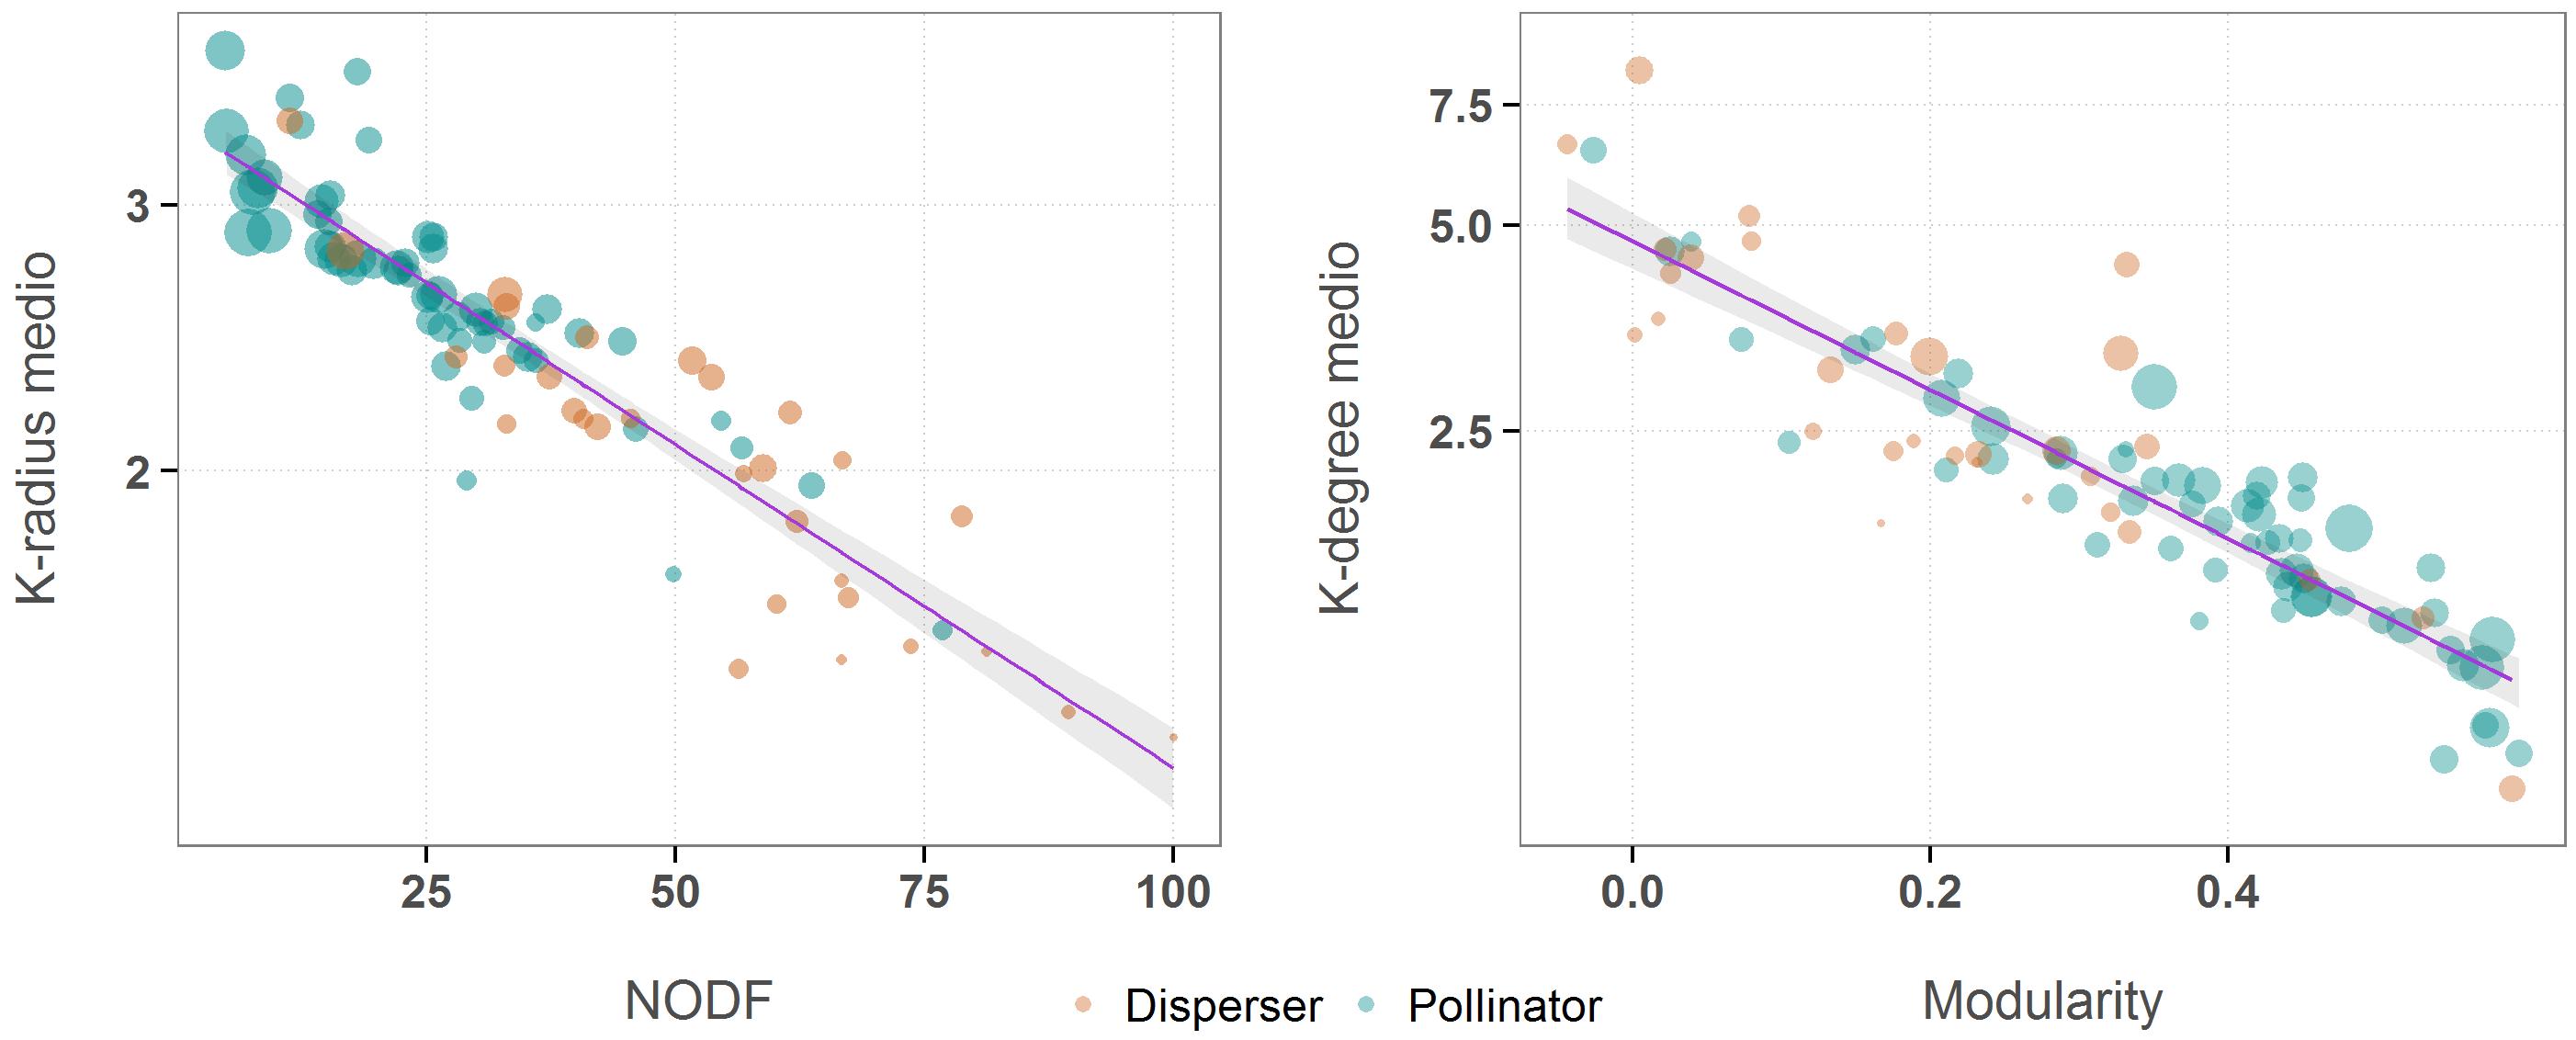
\includegraphics[scale=0.2]{ESTATICA_correlation_figs.png}
\caption {Diagrama de dispersión del $\overline {k}_{radius}$ respecto a $NODF$ (izquierda), y del $\overline {k}_{degree}$ respecto a la $Modularity$ (derecha). Cada punto es una red, su área es proporcional al logaritmo del número de especies y el color indica la clase de comunidad. Se han incluido las líneas de regresión con sus intervalos de confianza en sombreado.}
\label{fig:ESTATICA_corrfigs}
\end{figure}

Las nubes de puntos se representan sobre eje lineal en las abscisas y logarítmico en las ordenadas. Parecen compatibles con un modelo exponencial, así que procedimos a calcular las regresiones lineales $log(Y) ~ X$. Los resultados numéricos se resumen en la tabla \ref{table:table_lmodel}. Como muestra el valor ajustado de $R^2$ $(0,84)$, el logaritmo de $\overline {k}_{radius}$ tiene una correlación muy elevada con $NODF$. 
\begin{align}
\displaystyle \log({\overline k_{radius}}) = \beta_1 \times NODF + \beta_0
\stepcounter{equation}\tag{\theequation}\label{eq:kradius_vs_nodf}
\end{align}
Es sencillo de entender; si la red es muy anidada las especies se conectan directamente a las \textit{shells} más internas y su distancia a los nodos de la \textit{shell} máxima es pequeña. 

\begin{table}[ht]
\centering
\begin{tabular}{|l r | l r|}
\hline
$log(\overline {k}_{radius})$ vs $NODF$& & $log(\overline {k}_{degree})$ vs $Modularity$ & \\
\hline
$\beta_1$ & $-$0.0098 & $\beta'_1$ & -2.5031 \\
$\beta_0$ & 1.2269 & $\beta'_0$ & 1.5553 \\
$R^2$ ajustado&  0.8427  & $R'^2$ ajustado& 0.8064\\
p-value & $<2.2 \times 10^{-16}$& p-value' & $<2.2 \times 10^{-16}$\\
\hline
\end{tabular}
\caption{\label{table:table_lmodel} Resultados de las regresiones lineales}
\end{table}

La correlación entre $\overline {k}_{degree}$ y $Modularity$ es más complicada de intuir. La distribución de densidad del $k_{degree}$ está más concentrada y sesgada hacia la izquierda cuanto más modular es la red. En ese caso la mayoría de las especies tienen valores reducidos del ${k}_{degree}$ y en consecuencia el valor medio es reducido. La distribución se va aplanando a medida que la modularidad decrece y el valor medio se desplaza hacia la derecha. En la figura \ref{fig:ESTATICA_density_plots} se puede ver este efecto.

Si se examina de nuevo la figura \ref{fig:ESTATICA_corrfigs}, se verá que las redes de mayor tamaño son también las que tienen valores más altos de $Modularity$. La mayoría de ellas son de la clase \textit{planta-polinizador} mientras que las tipo \textit{dispersor de semillas} son más pequeñas. Este hecho ya fue apuntado por Olesen que estudió 51 redes y encontró que las que tienen menos de 150 especies no son modulares \cite{olesen2007modularity}. Los valores elevados de $\overline {k}_{degree}$ en redes reducidas casan bien con la observación de que en ese caso las especies se encuentran más próximas a la \textit{shell} más interna y añaden valores altos al ${k}_{degree}$ de las especies a las que se conectan.

\begin{figure}[h!]
\centering
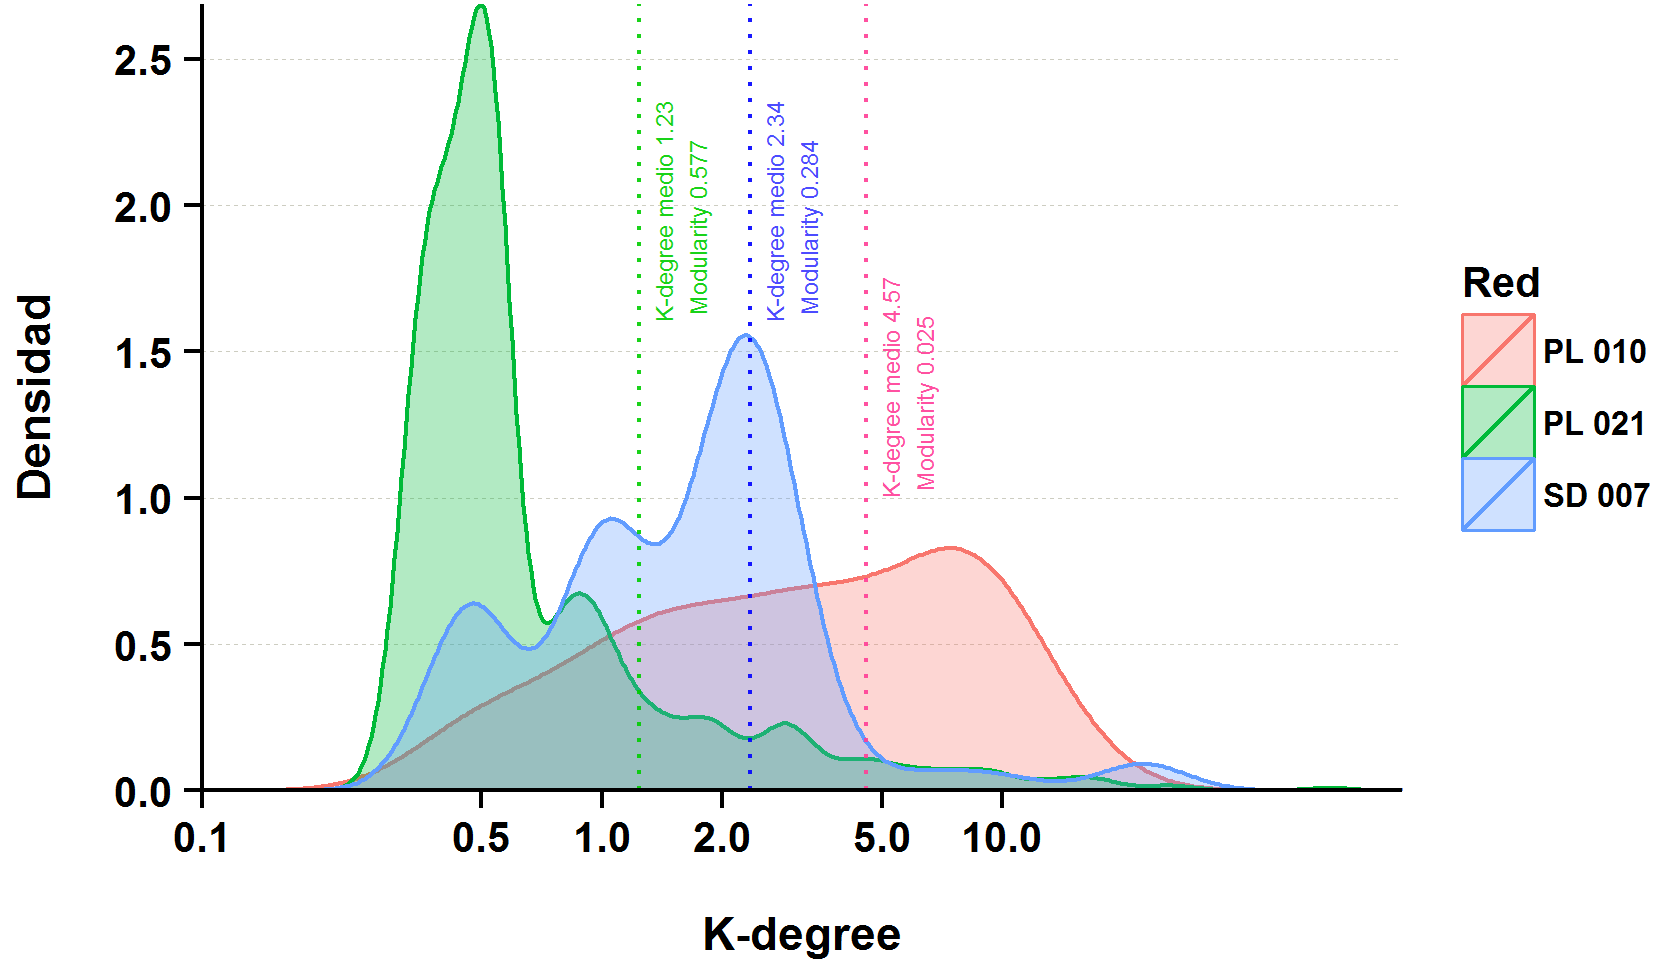
\includegraphics[scale=0.85]{Figures/ESTATICA_density_plots.png}
\caption {Distribución de densidad del $k_{degree}$ en tres redes diferentes. Junto a las líneas verticales pueden verse los valores del $\overline {k}_{degree}$ y de la $Modularity$.}
\label{fig:ESTATICA_density_plots}
\end{figure}

Las elevadas correlaciones de $\overline {k}_{radius}$ con $NODF$ y de $\overline {k}_{radius}$ con $Modularity$ son suficientes para esta investigación. Por ejemplo, no se propugna que $log(\overline {k}_{radius})$ sea un buen predictor de $NODF$, de hecho el test de \textit{Shapiro-Wilk} muestra heterocedasticidad. La colección de la \textit{Web of Life} no es una muestra aleatoria, y las distribuciones de las magnitudes no son normales. Sin embargo, las correlaciones apoyan la idea de que el $\overline {k}_{radius}$ es un indicador global de una propiedad similar al anidamiento, y el $\overline {k}_{degree}$ de modularidad y que la \textit{descomposición k-core} es una herramienta de interés para el estudio del mutualismo.

\subsection{Análisis de modelo nulo}

Mediante este análisis hemos estudiado como se comportan estadísticamente dos índices, $NODF$ y $\overline k_{radius}$. La razón de escoger estas dos magnitudes es la alta correlación que
muestran para toda la colección. La tabla \ref{table:table_results_zscores} contiene los índices reducidos.

Por lo que respecta a la medida de anidamiento $NODF$, el resultado concuerda con la literatura. Utilizando un modelo nulo restrictivo, como el que hemos empleado para las redes pesadas, solo $3$ de $32$ son significativamente anidadas. Se consideran así si su $zNODF$ está por encima de $2$ lo que equivale a una probabilidad de aparición aleatoria inferior al $5\%$.
La medida de la compacidad con $\overline {k}_{radius}$ es más restrictiva. De las $32$ redes solo una es significativamente compacta ($z\overline {k}_{radius} < 2$), la red de polinizadores $059$, que además es una de las tres que muestra $zNODF$ por encima de $2$.

\begin{figure}[h!]
\centering
\includegraphics[scale=0.35]{Figures/ESTATICA_zscores_all.eps}
\caption {Diagramas de dispersión de $z\overline k_{radius}$ y $zNODF$ para toda la colección de redes. A la izquierda, en azul, las redes pesadas. A la derecha, en salmón, las redes binarias.}
\label{fig:ESTATICA_zscore_all}
\end{figure}

La situación es opuesta para las redes binarias, para las que se ha usado un modelo nulo \textit{free free}. Las $57$ disponibles en la colección muestran anidamiento no debido al azar según el análisis. Para este subconjunto la compacidad también resulta ser menos común que el anidamiento, solo $27$ tienen un índice $z\overline {k}_{radius}$ inferior a $2$.

De estos datos concluimos que $\overline k_{radius}$ puede resultar una medida útil de la proximidad del conjunto de las especies de la red a su núcleo más conectado. Solo parte de las redes significativamente anidadas de la colección, según $zNODF$, resultan ser también compactas. La probabilidad de aparición aleatoria de esta propiedad es inferior a la del anidamiento.


\subsection{Recableado aleatorio}

La idea subyacente a este experimento es que las comunidades mutualistas adoptan configuraciones estables, anidadas y compactas. Al recablear de forma aleatoria un porcentaje de sus enlaces deben de llegar a un estado más desordenado (fig. \ref{fig:z_M_PL_012_rewire_Binary_ES_model_5}). En el apartado anterior hemos visto que la premisa de partida no es cierta para las redes pesadas si se utiliza un modelo nulo restrictivo. Hemos limitado el experimento a las que tienen matriz de interacción binaria, en las que sí puede admitirse.

\begin{figure}[h!]
\centering
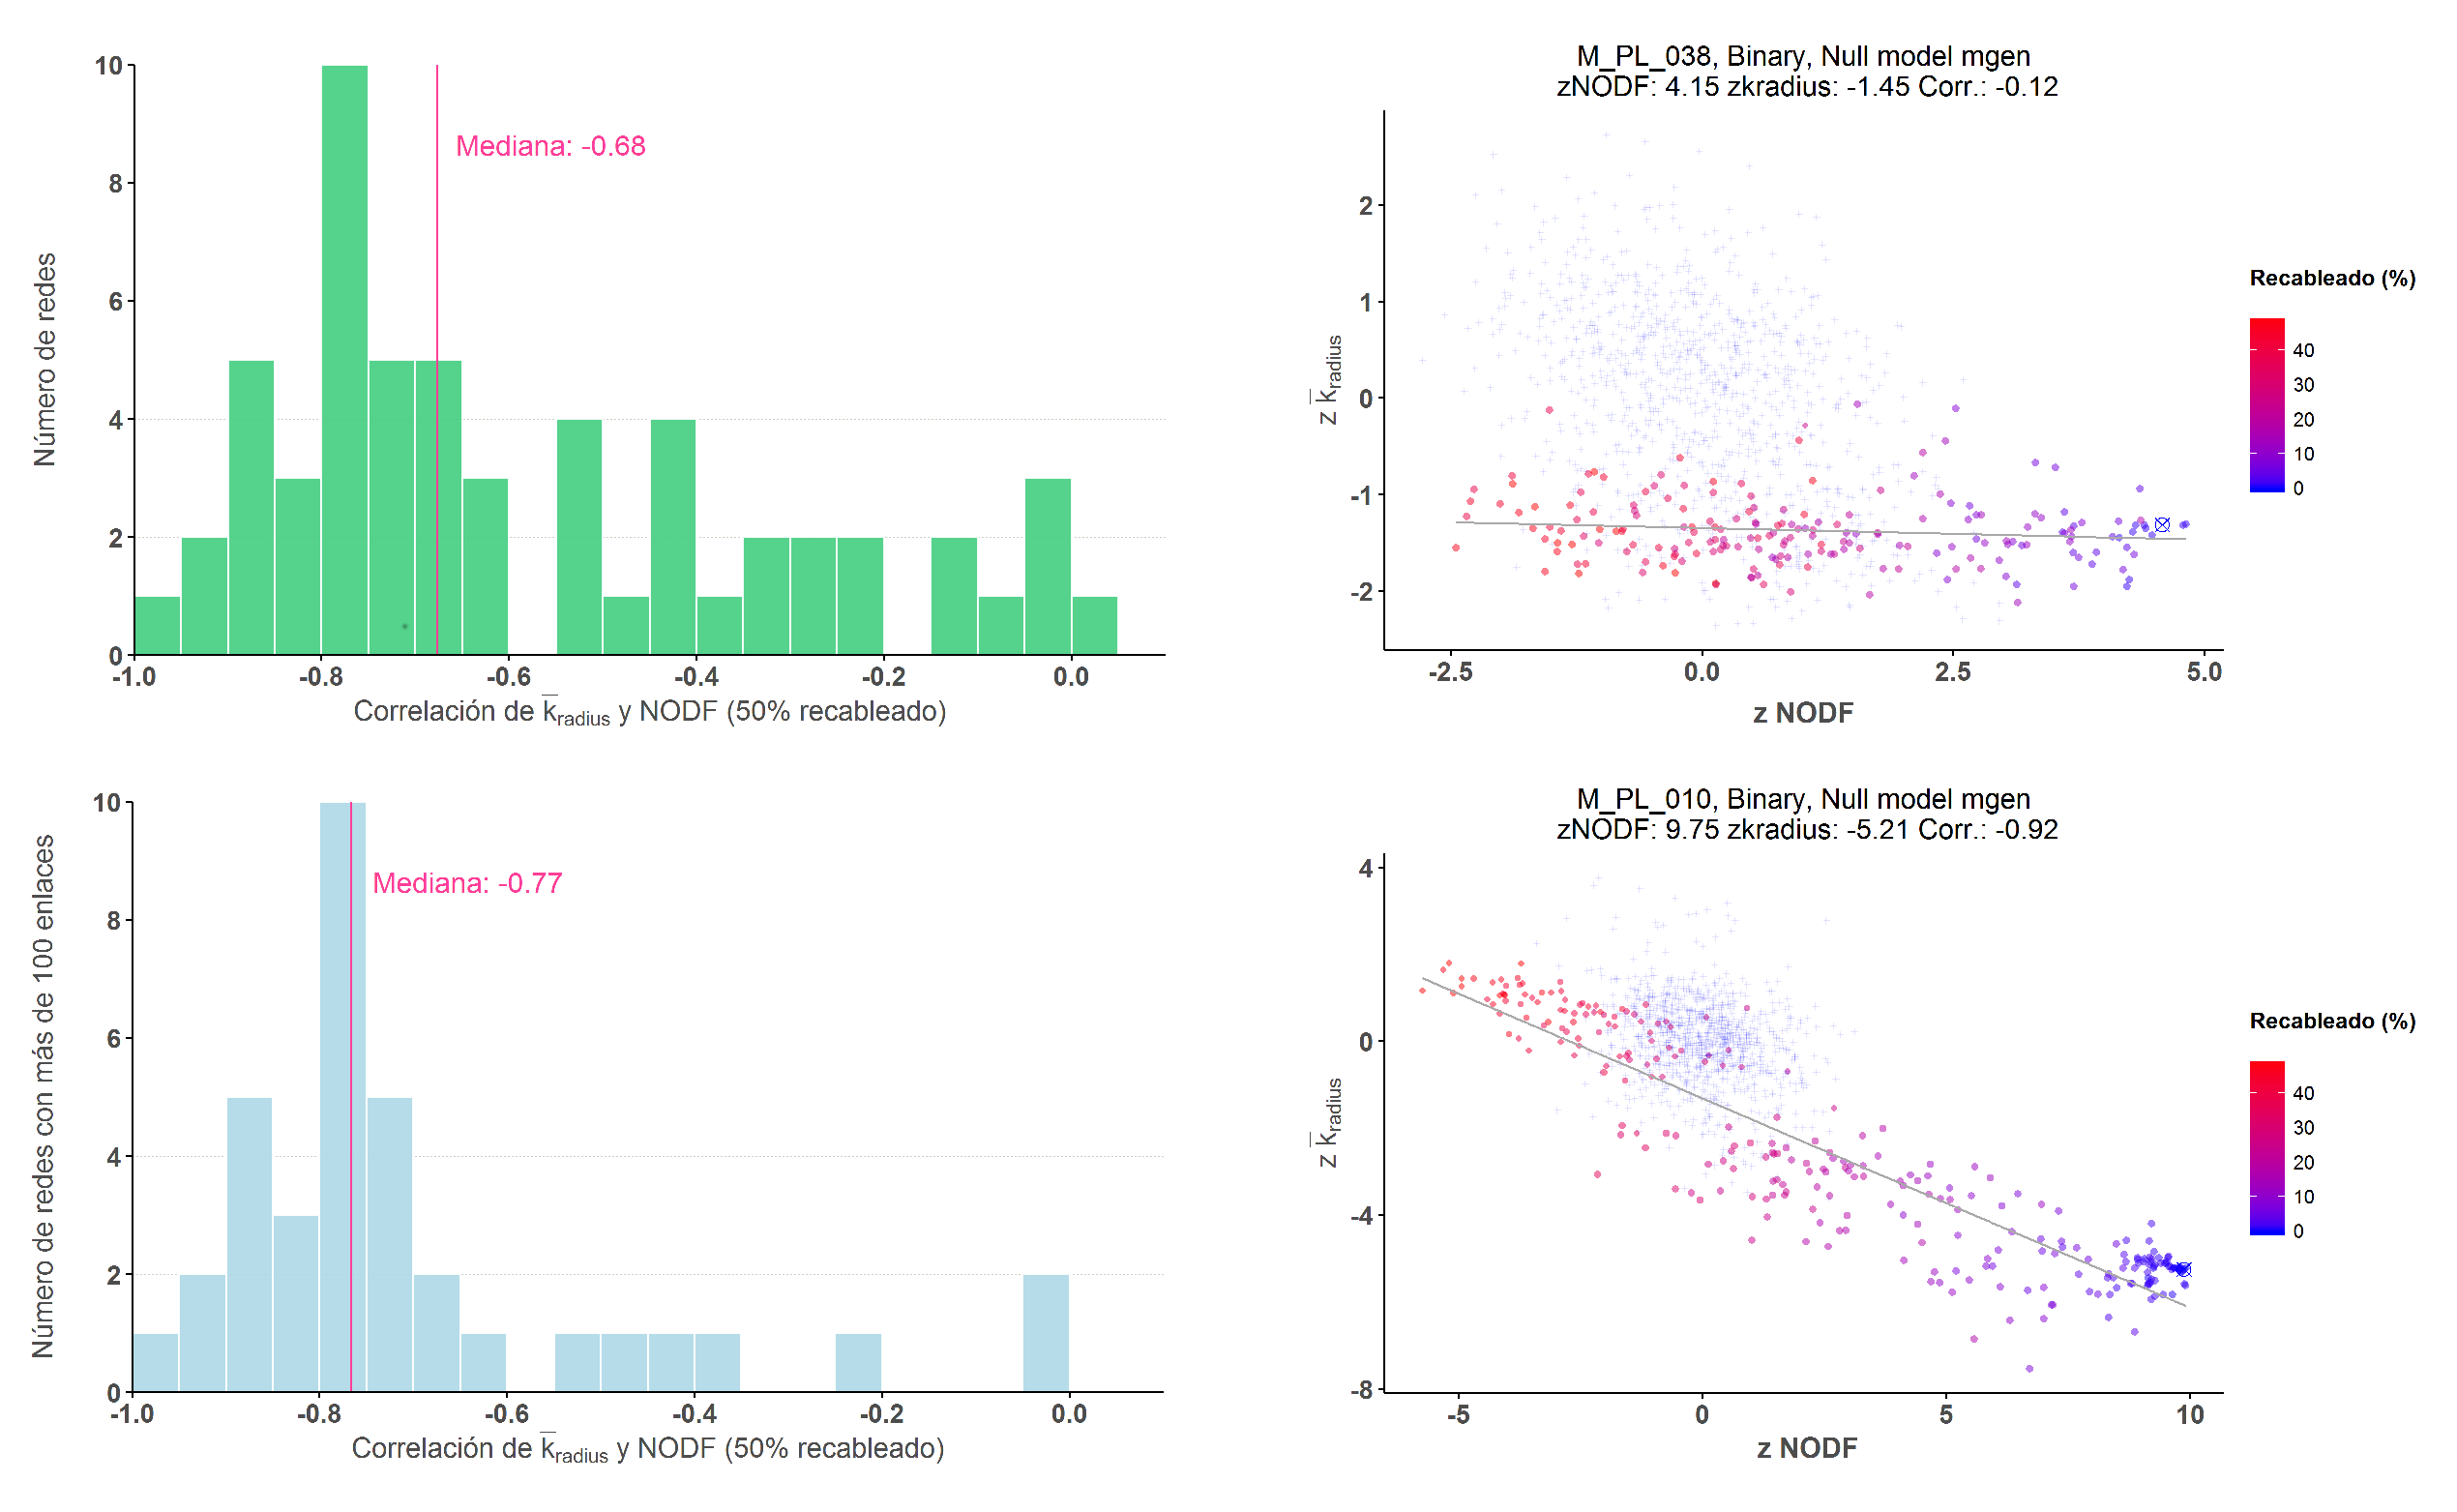
\includegraphics[scale=0.35]{Figures/ESTATICA_histo_corr_rewiring_ES.eps}
\caption {Experimento de recableado de las redes con matrices binarias. Histograma de correlación de los índices reducidos $z \overline {k}_{radius}$ y $zNODF$ para todas las redes (arriba) y para el subconjunto de las que tienen más de $100$ enlaces. En la columna de la derecha, resultados del experimento para las redes  $M\_PL\_038$ ($79$ enlaces, arriba) y $M\_PL\_038$ ($456$ enlaces, abajo).}
\label{fig:ESTATICA_histo_corr_rewiring}
\end{figure}

El histograma de la parte superior de la figura \ref{fig:ESTATICA_histo_corr_rewiring} muestra que los valores de la correlación se concentran en torno a $0.8$ lo que indica que ambas magnitudes se degradan en el mismo sentido al recablear, con un patrón similar. Sin embargo, hay un número no desdeñable para las que este valor es reducido e incluso próximo a $0$. El diagrama de recableado de la red $M\_PL\_038$ es un ejemplo, el anidamiento se destruye pero el $z \overline {k}_{radius}$ apenas se modifica. Una posible explicación es que la red inicialmente es anidada pero no compacta, de manera que
esta segunda magnitud ya presenta un alto grado inicial de desorden. También es una red pequeña, con una estructura más sensible a pequeños cambios.

En el histograma inferior se han eliminado las redes con menos de $100$ enlaces. La mayoría de las redes con bajos valores de correlación son de pequeño tamaño, la mediana se desplaza hasta $0,77$ y la distribución se parece más a una gaussiana. El diagrama de $M\_PL\_010$ muestra el comportamiento de las redes con más interacciones. La correlación es mucho mayor y el par de valores iniciales está más alejado de la nube de puntos del modelo nulo que en $M\_PL\_038$. La red $M\_PL\_010$ es fuertemente anidada y compacta. El recableado hace que los dos índices se degraden de forma similar y que pierda ambas propiedades aproximadamente a la vez.

\begin{figure}[h!]
\centering
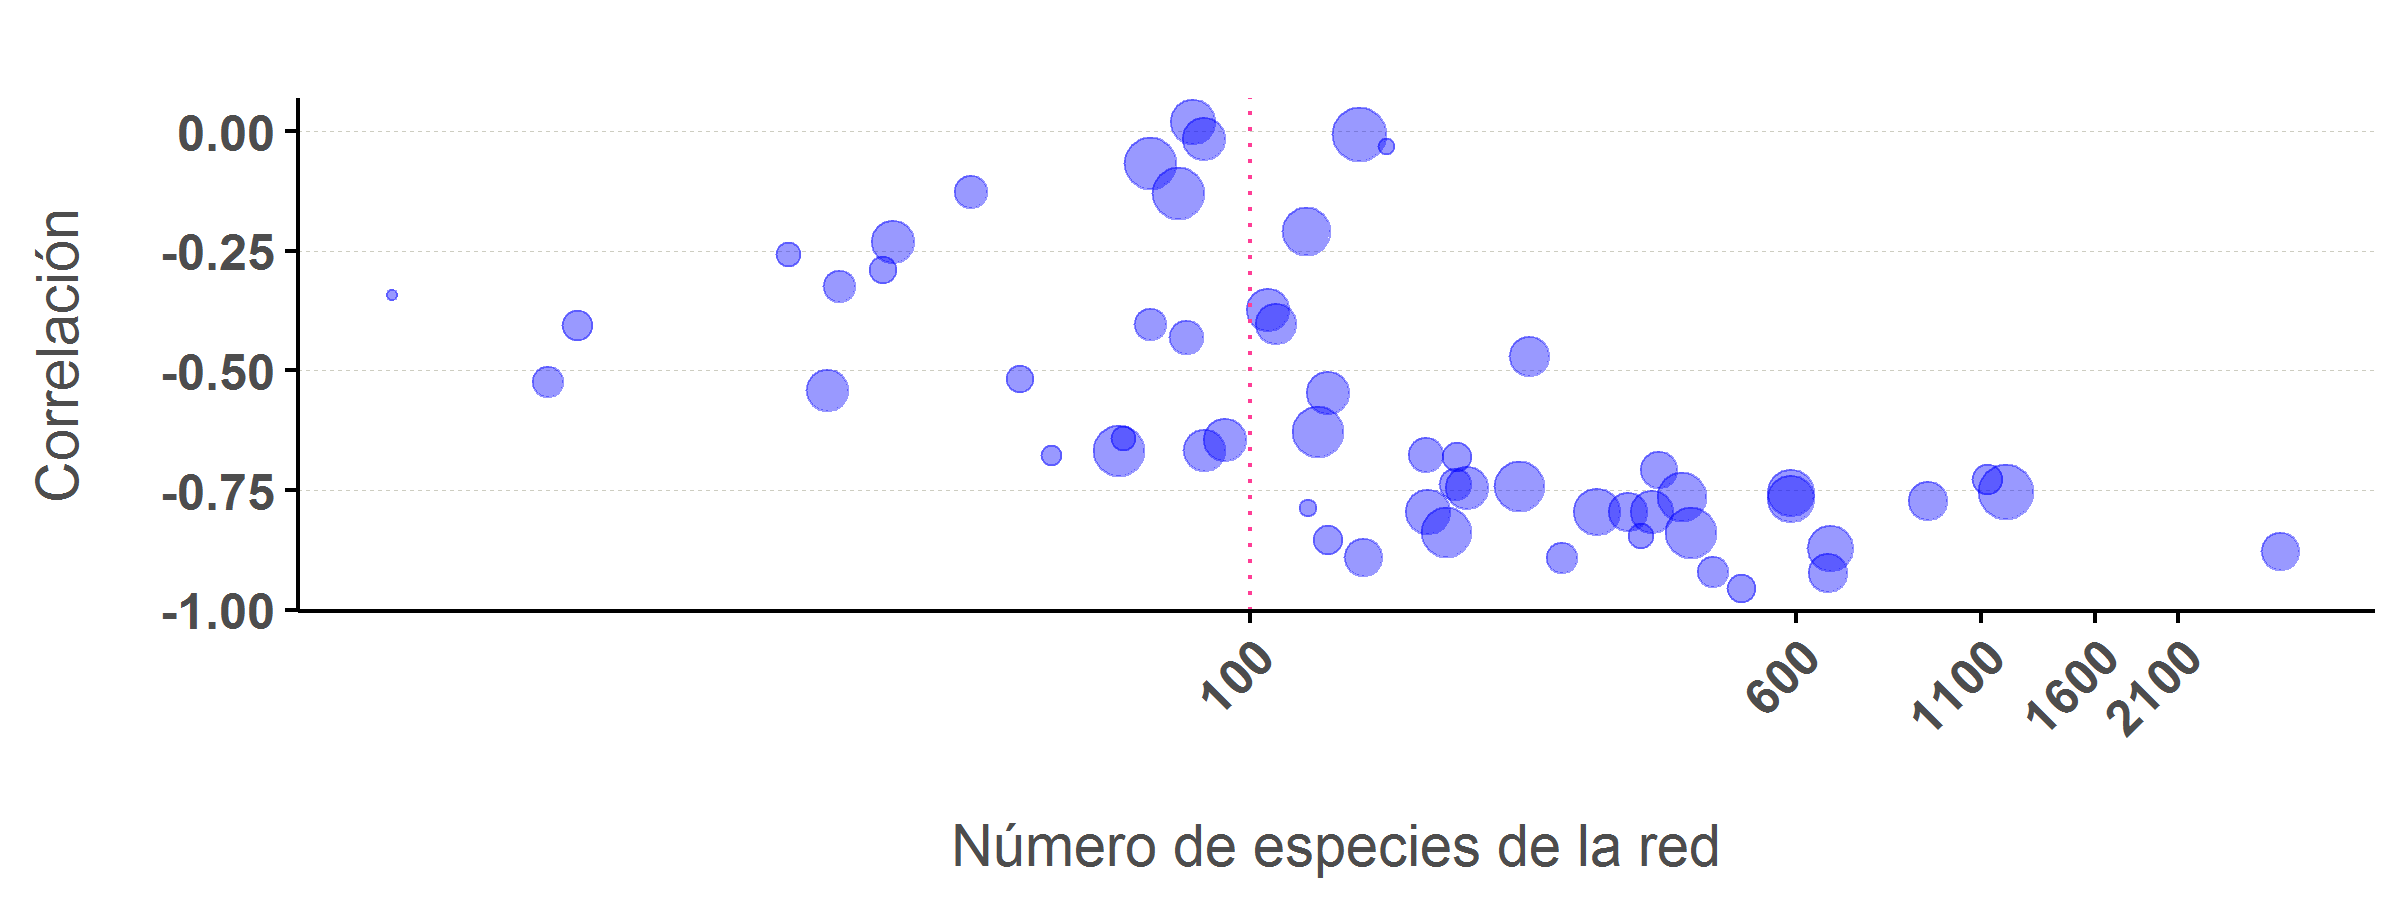
\includegraphics[scale=0.6]{Figures/ESTATITCA_asimetria_corr.png}
\caption {Correlación de $z \overline {k}_{radius}$ y $zNODF$ en función del número de especies de la red.}
\label{fig:ESTATICA_asimetria_corr}
\end{figure}

Buscando el origen de este comportamiento dispar, se ha representado el diagrama de dispersión que relaciona el valor de la correlación con el número de especies de la red y con la asimetría de clases. Esta se mide como el valor absoluto de la diferencia entre el número de especies de ambas clases dividida por su suma (tabla \ref{table:table_results_recableados}). El área correspondiente al círculo de cada especie es proporcional a esta cantidad. De la gráfica se deduce que cuanto mayor es el tamaño de la red la correlación lineal entre $NODF$ y $log(\overline {k}_{radius})$ tiene mayor tendencia a mantenerse aunque cambie un pequeño porcentaje de conexiones. Para redes más pequeñas, el factor que destruye con mayor rapidez el anidamiento es la asimetría, y la red $M\_SD\_007$ es un caso extremo, con $72$ especies de plantas, solo $7$ de polinizadores y una estructura muy peculiar como se verá en el próximo capítulo de visualizaciones. Estas redes asimétricas son mucho más sensibles a las reconexiones, porque hay una mayor probabilidad de alterar la \textit{k-shell} máxima.

Lo que muestra el experimento es que cuanto  mayores son el tamaño y la simetría, las redes parecen menos destructibles ante pequeños cambios. El valor de la correlación podría utilizarse como indicador numérico de la resistencia a una variación de las condiciones ambientales.

\begin{figure}[h!]
\centering
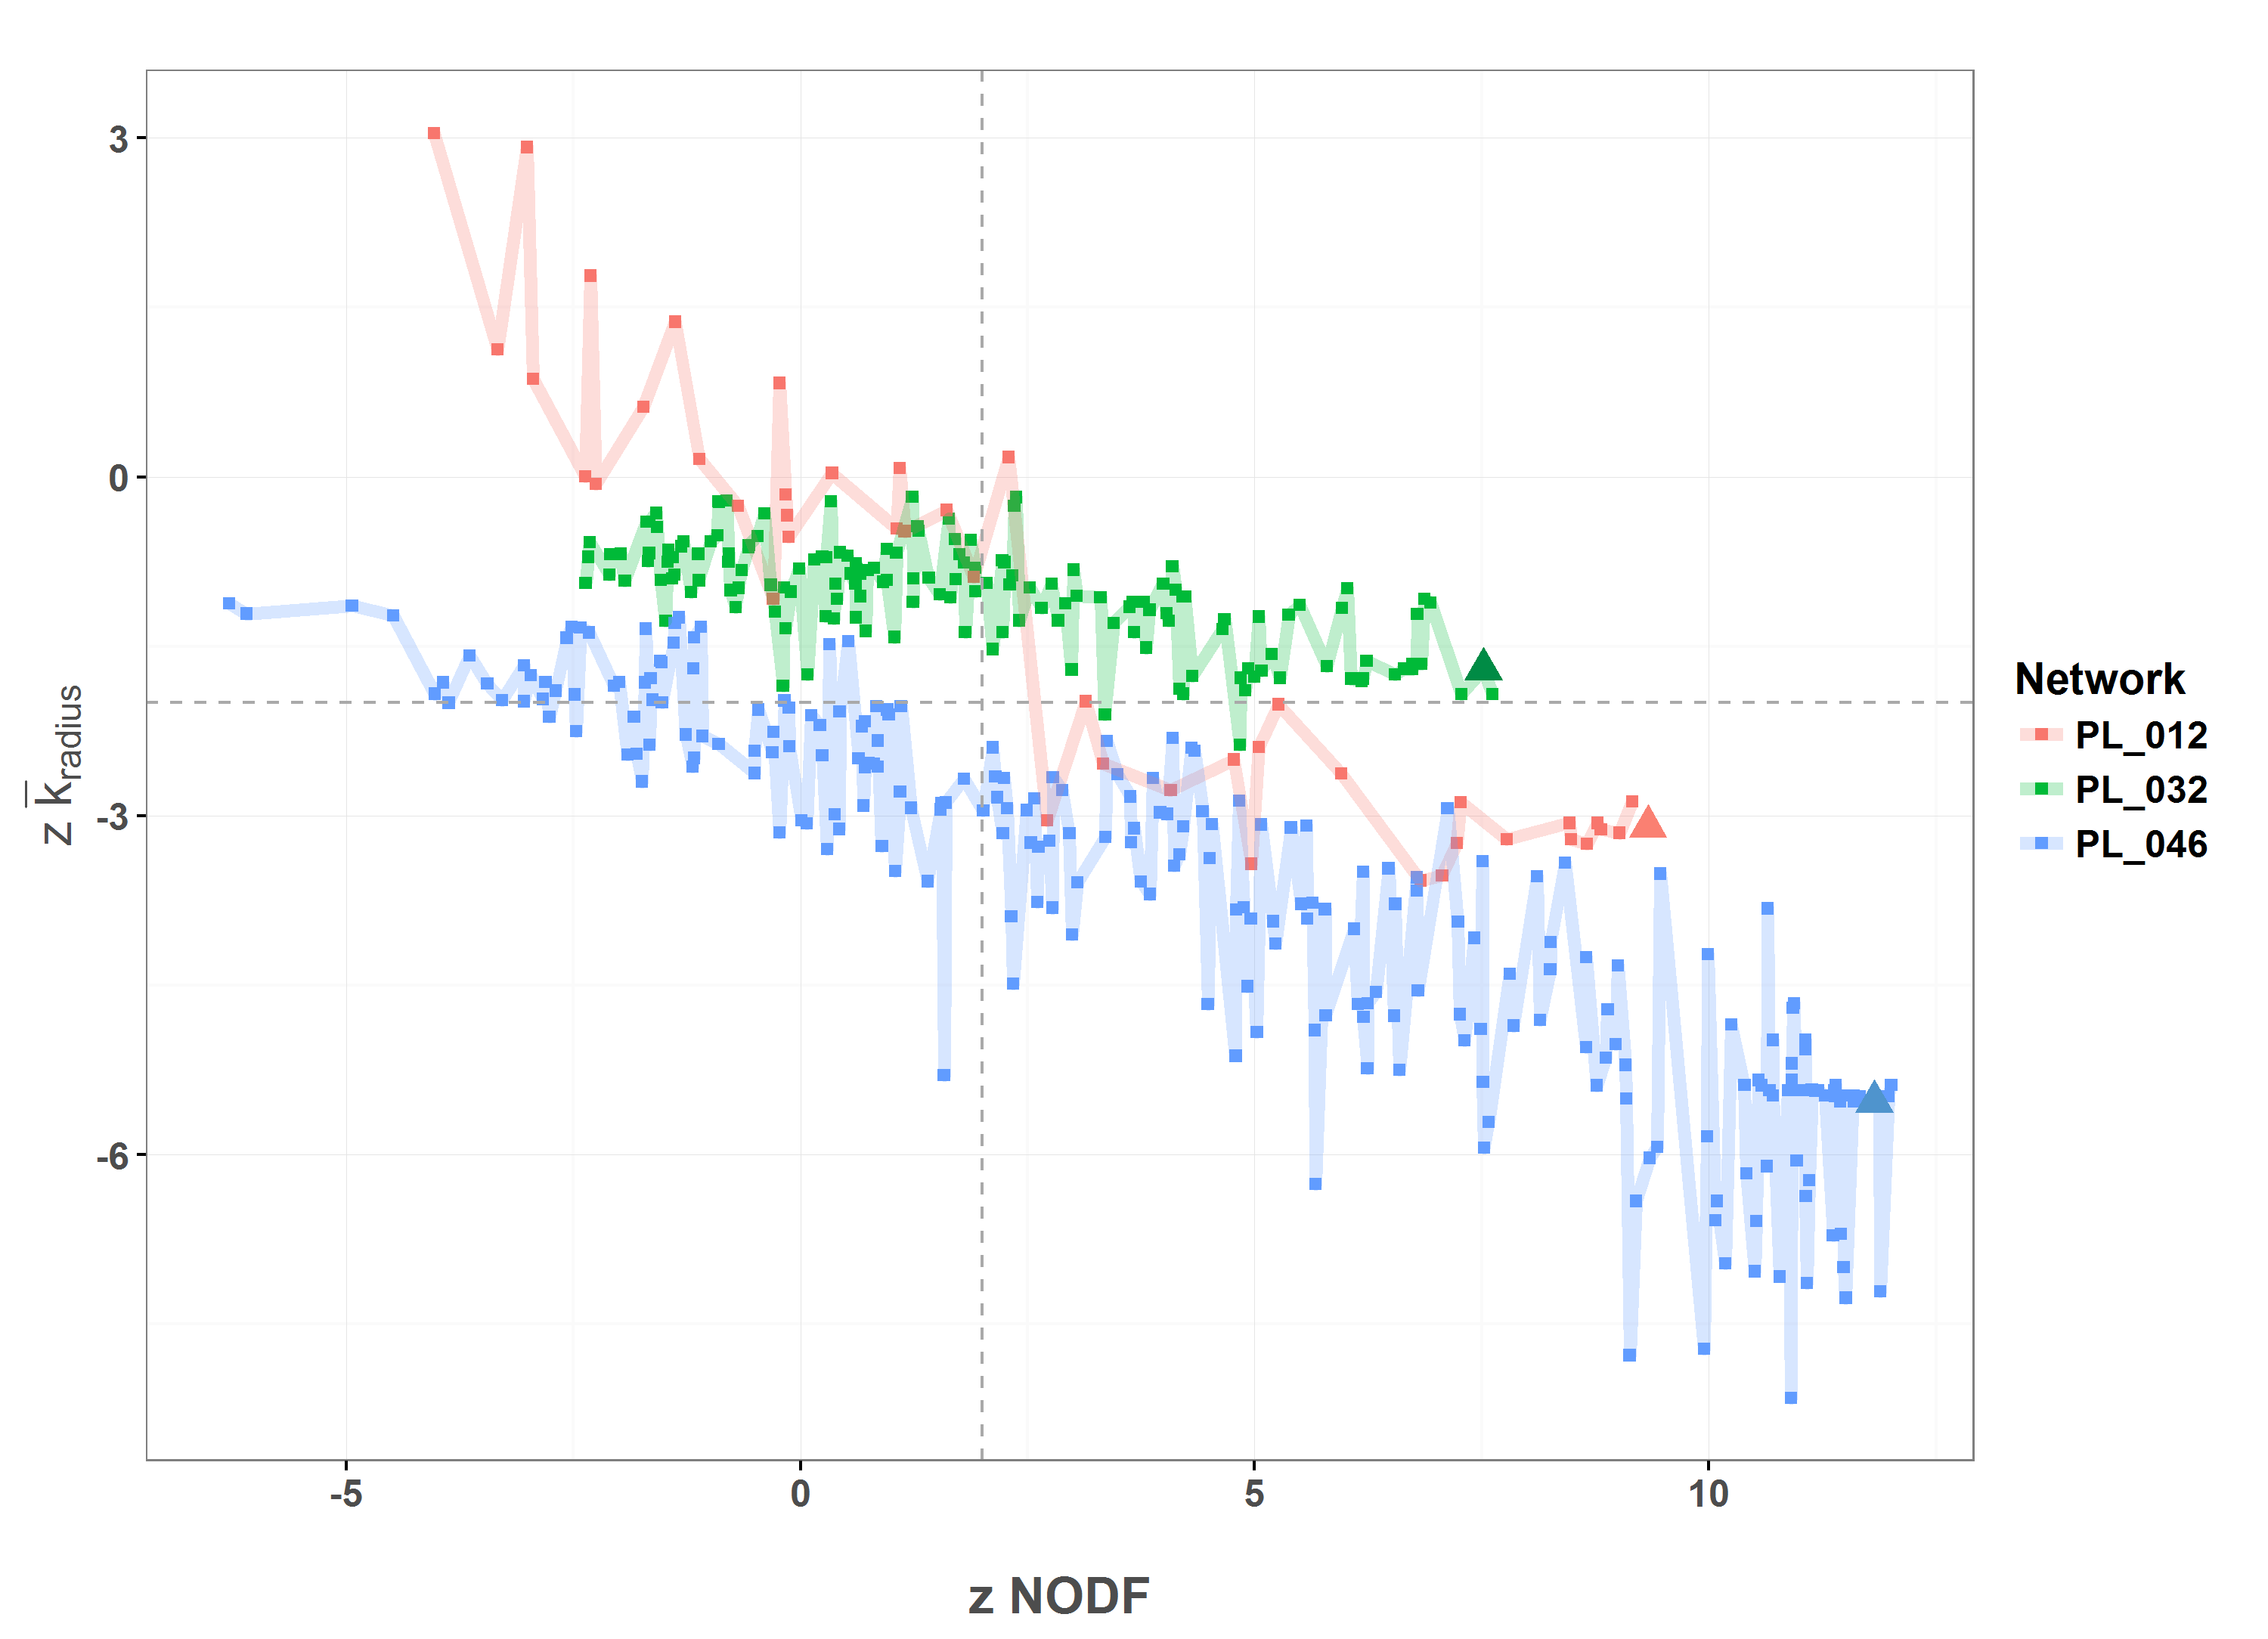
\includegraphics[scale=0.6]{ESTATICA_zscores_networks_evolution.png}
\caption {Comparativa de la evolución de $z \overline {k}_{radius}$ y $zNODF$ en el experimento de recableado de tres redes. Los triángulos marcan los pares de valores de las redes originales. A medida que crece el porcentaje de recableado aleatorio, las redes resultantes son más desordenadas y se desplazan al cuadrante superior izquierdo, combinación de falta de anidamiento y de compacidad.}
\label{fig:ESTATICA_asimetria_corr}
\end{figure}

\section{Conclusiones}

La \textit{descomposición k-core} proporciona una sólida base para el análisis del mutualismo. Hemos demostrado como las \textit{k-magnitudes} definidas como propiedades surgidas del procedimiento, permiten conocer en detalle la estructura de las redes. En particular, al promediar los valores locales para todo el sistema, $\overline {k}_{radius}$ y $\overline {k}_{degree}$ muestran una fuerte correlación con los observables globales $NODF$ y $Modularity$. 

Mediante el análisis de modelo nulo se ha comprobado que $\overline {k}_{radius}$ es una medida de compacidad, que es una propiedad que se presenta solo en un subconjunto de redes significativamente anidadas.

La descomposición es también útil para una nueva ordenación de importancia de las especies. El ${k}_{degree}$ permite refinar la que proporciona el grado, al crear una escala en la que hay una probabilidad muy inferior de repetición de valores.

Mediante el experimento de recableado hemos comprobado como el anidamiento y la compacidad desaparecen de forma casi simultánea en las redes binarias que parten de un estado muy ordenado. Este comportamiento es menos habitual en redes pequeñas o con una fuerte asimetría de especies.

Aunque hemos enfocado el estudio en redes mutualistas, la técnica se puede extender a otros tipos de redes bipartitas, por ejemplo comensalistas. Relaciones bipartitas y con fuerte anidamiento, como las que aparecen en redes de innovación y comercio, podrían también beneficiarse de este análisis.

\section{Anexo: Unidades reducidas}
\label{ESTATICA_ANEXO_zscores}
\begin{table}[ht!]
\fontsize{2.5mm}{2.5mm}\selectfont
  \centering
    \begin{tabular}{lrrrrrrrrr}
    \toprule
    $Red$  & $Matriz$ & $zNODF$ & $z\overline K_{radius}$ &  &  $Red$  & $Matriz$ & $zNODF$ & $z\overline K_{radius}$ \\
    \midrule
    M\_PL\_001 & Binaria & 10,58 & -2,33 &      & M\_PL\_046 & Binaria & 11,82 & -5,53 \\
    M\_PL\_002 & Binaria & 6,00 & -1,45 &      & M\_PL\_047 & Binaria & 13,07 & -1,98 \\
    M\_PL\_003 & Binaria & 5,87 & -1,05 &      & M\_PL\_048 & Binaria & 13,62 & -2,22 \\
    M\_PL\_004 & Pesada & 2,71 & 0,49 &      & M\_PL\_049 & Binaria & 10,53 & -3,83 \\
    M\_PL\_005 & Binaria & 11,77 & -2,87 &      & M\_PL\_050 & Binaria & 5,43 & -1,03 \\
    M\_PL\_006 & Pesada & -4,40 & 2,75 &      & M\_PL\_051 & Pesada & -1,01 & -0,40 \\
    M\_PL\_007 & Pesada & -7,66 & 1,61 &      & M\_PL\_052 & Binaria & 5,66 & -1,30 \\
    M\_PL\_008 & Binaria & 5,48 & -2,74 &      & M\_PL\_053 & Binaria & 5,05 & 0,00 \\
    M\_PL\_009 & Binaria & 5,97 & -3,10 &      & M\_PL\_054 & Pesada & -5,25 & 1,31 \\
    M\_PL\_010 & Binaria & 9,88 & -5,25 &      & M\_PL\_055 & Pesada & -2,51 & 0,30 \\
    M\_PL\_011 & Binaria & 5,68 & -1,40 &      & M\_PL\_056 & Pesada & -5,93 & 5,10 \\
    M\_PL\_012 & Binaria & 9,33 & -3,09 &      & M\_PL\_057 & Pesada & -5,94 & -1,92 \\
    M\_PL\_013 & Pesada & -2,26 & 0,69 &      & M\_PL\_058 & Pesada & -4,54 & 1,12 \\
    M\_PL\_014 & Binaria & 7,22 & -0,50 &      & M\_PL\_059 & Pesada & 6,84 & -7,34 \\
    M\_PL\_015 & Binaria & 15,16 & -1,56 &      & M\_SD\_001 & Pesada & -1,03 & 0,76 \\
    M\_PL\_016 & Binaria & 9,05 & -1,59 &      & M\_SD\_002 & Pesada & 0,16 & -1,50 \\
    M\_PL\_017 & Pesada & -5,09 & 2,13 &      & M\_SD\_003 & Pesada & 0,59 & 1,04 \\
    M\_PL\_018 & Binaria & 7,64 & -2,23 &      & M\_SD\_004 & Pesada & 0,17 & -1,79 \\
    M\_PL\_019 & Pesada & -4,33 & 1,60 &      & M\_SD\_005 & Pesada & 0,89 & -0,64 \\
    M\_PL\_020 & Binaria & 10,14 & -2,05 &      & M\_SD\_006 & Pesada & -1,47 & 1,06 \\
    M\_PL\_021 & Binaria & 8,06 & -2,53 &      & M\_SD\_007 & Binaria & 9,66 & 0,20 \\
    M\_PL\_022 & Binaria & 3,93 & 0,58 &      & M\_SD\_008 & Pesada & 0,09 & -1,24 \\
    M\_PL\_023 & Binaria & 6,32 & -2,84 &      & M\_SD\_009 & Pesada & -1,90 & 0,22 \\
    M\_PL\_024 & Pesada & -1,79 & -1,98 &      & M\_SD\_010 & Pesada & -3,64 & 0,55 \\
    M\_PL\_025 & Pesada & -3,04 & 0,46 &      & M\_SD\_011 & Binaria & 4,07 & -1,56 \\
    M\_PL\_026 & Binaria & 12,06 & -3,44 &      & M\_SD\_012 & Pesada & -0,24 & 2,74 \\
    M\_PL\_027 & Binaria & 3,94 & -1,29 &      & M\_SD\_013 & Binaria & 4,68 & -1,56 \\
    M\_PL\_028 & Binaria & 7,86 & -2,27 &      & M\_SD\_014 & Binaria & 10,53 & -5,39 \\
    M\_PL\_029 & Binaria & 7,70 & -2,76 &      & M\_SD\_015 & Binaria & 6,54 & -5,45 \\
    M\_PL\_030 & Binaria & 3,23 & -1,69 &      & M\_SD\_016 & Binaria & 16,65 & -7,99 \\
    M\_PL\_031 & Binaria & 3,98 & 0,22 &      & M\_SD\_017 & Binaria & 5,01 & -5,06 \\
    M\_PL\_032 & Binaria & 7,51 & -1,70 &      & M\_SD\_018 & Binaria & 3,77 & -1,35 \\
    M\_PL\_033 & Pesada & -2,26 & 2,05 &      & M\_SD\_019 & Binaria & 15,38 & -3,49 \\
    M\_PL\_034 & Binaria & 9,98 & -1,38 &      & M\_SD\_020 & Pesada & -0,17 & 2,60 \\
    M\_PL\_035 & Binaria & 9,55 & -1,90 &      & M\_SD\_021 & Binaria & 9,74 & -2,15 \\
    M\_PL\_036 & Binaria & 3,01 & -0,91 &      & M\_SD\_022 & Binaria & 13,24 & -2,40 \\
    M\_PL\_037 & Binaria & 3,99 & -1,54 &      & M\_SD\_023 & Pesada & 4,09 & -0,73 \\
    M\_PL\_038 & Binaria & 4,58 & -1,31 &      & M\_SD\_024 & Binaria & 4,17 & -0,91 \\
    M\_PL\_039 & Binaria & 5,69 & -1,95 &      & M\_SD\_025 & Binaria & 3,52 & -2,34 \\
    M\_PL\_040 & Pesada & -3,66 & 3,03 &      & M\_SD\_026 & Binaria & 2,58 & -1,28 \\
    M\_PL\_041 & Pesada & -1,61 & -0,42 &      & M\_SD\_027 & Binaria & 4,51 & -3,14 \\
    M\_PL\_042 & Binaria & 3,20 & -2,53 &      & M\_SD\_028 & Binaria & 4,84 & -3,29 \\
    M\_PL\_043 & Binaria & 6,87 & -1,03 &      & M\_SD\_029 & Binaria & 3,21 & -0,96 \\
    M\_PL\_044 & Pesada & -3,26 & 0,65 &      & M\_SD\_030 & Binaria & 2,45 & -1,13 \\
    M\_PL\_045 & Pesada & -1,93 & 1,00 &      &      &      &      &  \\
    \bottomrule
    \end{tabular}%
    \caption{\label{table:table_results_zscores} Resultados del análisis de modelo nulo en unidades reducidas.}
\end{table}%


\clearpage
\section{Anexo: K-magnitudes de las redes analizadas}
\label{ESTATICA_ANEXO_kmagnitudes}
\begin{table}[ht!]
\fontsize{2.2mm}{2.2mm}\selectfont
  \centering
    \begin{tabular}{lrrrrrrrrr}
    \toprule
    $Red$  & $Matriz$ & $Pl.$ & $Anim.$ & $Enlaces$ & $k_{max}$ & $\overline k_{degree}$ & $\overline k_{radius}$ & $NODF$ & $Modul.$ \\
    \midrule
     M\_PL\_001 & Binaria & 84   & 101  & 361  & 4    & 1,56 & 3,01 & 14,46 & 0,45 \\
    M\_PL\_002 & Binaria & 43   & 64   & 196  & 3    & 1,40 & 3,04 & 15,36 & 0,48 \\
    M\_PL\_003 & Binaria & 36   & 25   & 81   & 2    & 0,93 & 3,31 & 19,19 & 0,57 \\
    M\_PL\_004 & Pesada & 12   & 102  & 167  & 3    & 1,52 & 2,53 & 28,15 & 0,45 \\
    M\_PL\_005 & Binaria & 96   & 275  & 923  & 8    & 2,54 & 2,80 & 14,74 & 0,24 \\
    M\_PL\_006 & Pesada & 17   & 61   & 146  & 4    & 2,28 & 2,44 & 44,58 & 0,33 \\
    M\_PL\_007 & Pesada & 16   & 36   & 85   & 3    & 1,68 & 2,51 & 31,54 & 0,36 \\
    M\_PL\_008 & Binaria & 11   & 38   & 106  & 4    & 2,19 & 2,37 & 35,97 & 0,21 \\
    M\_PL\_009 & Binaria & 24   & 118  & 242  & 4    & 1,54 & 2,81 & 15,39 & 0,44 \\
    M\_PL\_010 & Binaria & 31   & 76   & 456  & 8    & 4,57 & 2,38 & 35,17 & 0,02 \\
    M\_PL\_011 & Binaria & 14   & 13   & 52   & 3    & 2,27 & 2,16 & 54,59 & 0,29 \\
    M\_PL\_012 & Binaria & 29   & 55   & 145  & 4    & 2,01 & 2,51 & 30,40 & 0,42 \\
    M\_PL\_013 & Pesada & 9    & 56   & 103  & 4    & 1,96 & 2,40 & 34,25 & 0,38 \\
    M\_PL\_014 & Binaria & 29   & 81   & 179  & 3    & 1,48 & 2,80 & 25,68 & 0,44 \\
    M\_PL\_015 & Binaria & 131  & 666  & 2933 & 9    & 2,90 & 2,88 & 9,17 & 0,35 \\
    M\_PL\_016 & Binaria & 26   & 179  & 412  & 5    & 1,88 & 2,73 & 21,98 & 0,42 \\
    M\_PL\_017 & Pesada & 25   & 79   & 299  & 6    & 3,28 & 2,47 & 40,37 & 0,15 \\
    M\_PL\_018 & Binaria & 39   & 105  & 383  & 5    & 2,26 & 2,74 & 19,73 & 0,24 \\
    M\_PL\_019 & Pesada & 40   & 85   & 264  & 5    & 1,97 & 2,71 & 17,51 & 0,34 \\
    M\_PL\_020 & Binaria & 20   & 91   & 190  & 4    & 1,84 & 2,56 & 37,12 & 0,39 \\
    M\_PL\_021 & Binaria & 91   & 677  & 1193 & 5    & 1,23 & 3,06 & 7,55 & 0,58 \\
    M\_PL\_022 & Binaria & 21   & 45   & 83   & 2    & 0,84 & 3,68 & 18,02 & 0,60 \\
    M\_PL\_023 & Binaria & 23   & 72   & 125  & 3    & 1,35 & 2,75 & 22,88 & 0,54 \\
    M\_PL\_024 & Pesada & 11   & 18   & 38   & 3    & 1,71 & 1,97 & 29,02 & 0,42 \\
    M\_PL\_025 & Pesada & 13   & 44   & 143  & 5    & 3,40 & 2,13 & 46,02 & 0,16 \\
    M\_PL\_026 & Binaria & 105  & 54   & 204  & 3    & 1,13 & 2,85 & 25,13 & 0,56 \\
    M\_PL\_027 & Binaria & 18   & 60   & 120  & 3    & 1,20 & 2,96 & 13,94 & 0,55 \\
    M\_PL\_028 & Binaria & 41   & 139  & 374  & 5    & 2,11 & 2,75 & 16,43 & 0,37 \\
    M\_PL\_029 & Binaria & 49   & 118  & 346  & 5    & 1,94 & 2,76 & 15,77 & 0,41 \\
    M\_PL\_030 & Binaria & 28   & 53   & 109  & 2    & 0,83 & 3,54 & 11,16 & 0,54 \\
    M\_PL\_031 & Binaria & 48   & 49   & 156  & 4    & 1,57 & 3,39 & 12,34 & 0,54 \\
    M\_PL\_032 & Binaria & 7    & 33   & 65   & 3    & 2,41 & 2,07 & 56,66 & 0,10 \\
    M\_PL\_033 & Pesada & 13   & 34   & 141  & 5    & 3,40 & 2,24 & 29,50 & 0,07 \\
    M\_PL\_034 & Binaria & 26   & 128  & 312  & 5    & 2,10 & 2,61 & 25,01 & 0,42 \\
    M\_PL\_035 & Binaria & 61   & 36   & 178  & 4    & 1,74 & 2,85 & 25,74 & 0,43 \\
    M\_PL\_036 & Binaria & 10   & 12   & 30   & 2    & 1,31 & 2,51 & 35,96 & 0,38 \\
    M\_PL\_037 & Binaria & 10   & 40   & 72   & 3    & 1,37 & 2,70 & 23,16 & 0,44 \\
    M\_PL\_038 & Binaria & 8    & 42   & 79   & 3    & 1,56 & 2,44 & 28,31 & 0,39 \\
    M\_PL\_039 & Binaria & 17   & 51   & 129  & 4    & 1,99 & 2,61 & 25,34 & 0,45 \\
    M\_PL\_040 & Pesada & 29   & 43   & 114  & 3    & 1,32 & 2,92 & 15,18 & 0,50 \\
    M\_PL\_041 & Pesada & 31   & 43   & 145  & 4    & 2,11 & 2,51 & 25,30 & 0,35 \\
    M\_PL\_042 & Binaria & 12   & 6    & 25   & 3    & 2,34 & 1,71 & 49,79 & 0,33 \\
    M\_PL\_043 & Binaria & 28   & 82   & 250  & 4    & 1,99 & 2,71 & 22,17 & 0,29 \\
    M\_PL\_044 & Pesada & 110  & 609  & 1125 & 4    & 1,12 & 3,36 & 4,92 & 0,57 \\
    M\_PL\_045 & Pesada & 17   & 26   & 63   & 3    & 1,73 & 2,43 & 30,77 & 0,45 \\
    M\_PL\_046 & Binaria & 16   & 44   & 278  & 8    & 6,45 & 1,96 & 63,60 & -0,03 \\
    M\_PL\_047 & Binaria & 19   & 186  & 425  & 6    & 2,31 & 2,56 & 29,96 & 0,29 \\
    M\_PL\_048 & Binaria & 30   & 236  & 671  & 7    & 2,78 & 2,61 & 26,23 & 0,21 \\
    M\_PL\_049 & Binaria & 37   & 225  & 590  & 6    & 2,08 & 2,76 & 18,13 & 0,38 \\
    M\_PL\_050 & Binaria & 14   & 35   & 86   & 3    & 1,71 & 2,49 & 32,58 & 0,43 \\
    M\_PL\_051 & Pesada & 14   & 90   & 164  & 4    & 2,13 & 2,34 & 26,96 & 0,45 \\
    M\_PL\_052 & Binaria & 15   & 39   & 92   & 3    & 1,70 & 2,51 & 30,91 & 0,31 \\
    M\_PL\_053 & Binaria & 99   & 294  & 589  & 3    & 0,92 & 3,80 & 4,71 & 0,58 \\
    M\_PL\_054 & Pesada & 113  & 318  & 773  & 5    & 1,42 & 3,07 & 8,08 & 0,46 \\
    M\_PL\_055 & Pesada & 64   & 195  & 431  & 4    & 1,29 & 3,13 & 8,71 & 0,52 \\
    M\_PL\_056 & Pesada & 91   & 365  & 871  & 5    & 1,43 & 3,24 & 6,86 & 0,46 \\
    M\_PL\_057 & Pesada & 114  & 883  & 1920 & 8    & 1,80 & 2,88 & 7,04 & 0,48 \\
    M\_PL\_058 & Pesada & 32   & 81   & 319  & 6    & 3,03 & 2,48 & 26,64 & 0,22 \\
    M\_PL\_059 & Pesada & 13   & 13   & 71   & 5    & 4,72 & 1,57 & 76,88 & 0,04 \\
    M\_SD\_001 & Pesada & 7    & 21   & 50   & 3    & 2,33 & 2,16 & 40,77 & 0,18 \\
    M\_SD\_002 & Pesada & 31   & 9    & 119  & 6    & 4,61 & 1,85 & 62,16 & 0,02 \\
    M\_SD\_003 & Pesada & 25   & 16   & 68   & 3    & 1,78 & 2,45 & 41,09 & 0,33 \\
    M\_SD\_004 & Pesada & 34   & 20   & 95   & 4    & 2,37 & 2,19 & 39,82 & 0,35 \\
    M\_SD\_005 & Pesada & 25   & 13   & 49   & 3    & 1,33 & 2,38 & 27,93 & 0,53 \\
    M\_SD\_006 & Pesada & 21   & 15   & 51   & 3    & 1,51 & 2,35 & 32,79 & 0,45 \\
    M\_SD\_007 & Binaria & 72   & 7    & 143  & 3    & 2,34 & 2,37 & 51,67 & 0,28 \\
    M\_SD\_008 & Pesada & 16   & 10   & 110  & 7    & 6,56 & 1,48 & 56,33 & -0,04 \\
    M\_SD\_009 & Pesada & 7    & 18   & 38   & 3    & 1,90 & 2,15 & 33,02 & 0,32 \\
    M\_SD\_010 & Pesada & 50   & 14   & 234  & 6    & 4,48 & 2,14 & 42,13 & 0,04 \\
    M\_SD\_011 & Binaria & 11   & 14   & 47   & 3    & 2,14 & 2,17 & 45,41 & 0,31 \\
    M\_SD\_012 & Pesada & 35   & 29   & 146  & 4    & 2,31 & 2,57 & 33,04 & 0,23 \\
    M\_SD\_013 & Binaria & 36   & 19   & 197  & 7    & 4,38 & 2,31 & 37,37 & 0,33 \\
    M\_SD\_014 & Binaria & 16   & 17   & 121  & 5    & 5,16 & 1,87 & 78,76 & 0,08 \\
    M\_SD\_015 & Binaria & 5    & 27   & 86   & 4    & 4,25 & 1,65 & 67,34 & 0,03 \\
    M\_SD\_016 & Binaria & 24   & 61   & 500  & 11   & 8,40 & 2,01 & 58,84 & 0,00 \\
    M\_SD\_017 & Binaria & 16   & 8    & 72   & 5    & 4,74 & 1,63 & 60,12 & 0,08 \\
    M\_SD\_018 & Binaria & 29   & 32   & 66   & 2    & 0,75 & 3,41 & 11,21 & 0,59 \\
    M\_SD\_019 & Binaria & 169  & 40   & 666  & 7    & 3,23 & 2,62 & 32,87 & 0,33 \\
    M\_SD\_020 & Pesada & 25   & 33   & 150  & 5    & 3,07 & 2,31 & 53,55 & 0,13 \\
    M\_SD\_021 & Binaria & 18   & 28   & 129  & 5    & 3,46 & 2,19 & 61,52 & 0,18 \\
    M\_SD\_022 & Binaria & 207  & 110  & 1121 & 8    & 3,21 & 2,80 & 16,81 & 0,20 \\
    M\_SD\_023 & Pesada & 15   & 8    & 38   & 3    & 2,30 & 2,03 & 66,80 & 0,22 \\
    M\_SD\_024 & Binaria & 12   & 7    & 40   & 3    & 2,50 & 1,99 & 56,83 & 0,12 \\
    M\_SD\_025 & Binaria & 7    & 6    & 22   & 3    & 2,41 & 1,69 & 66,67 & 0,19 \\
    M\_SD\_026 & Binaria & 3    & 3    & 6    & 2    & 1,83 & 1,33 & 100,00 & 0,17 \\
    M\_SD\_027 & Binaria & 12   & 4    & 31   & 4    & 3,45 & 1,53 & 73,61 & 0,00 \\
    M\_SD\_028 & Binaria & 8    & 5    & 26   & 4    & 3,65 & 1,38 & 89,47 & 0,02 \\
    M\_SD\_029 & Binaria & 4    & 5    & 10   & 2    & 1,98 & 1,52 & 81,25 & 0,27 \\
    M\_SD\_030 & Binaria & 5    & 4    & 11   & 2    & 2,24 & 1,50 & 66,67 & 0,23 \\
    \bottomrule
    \end{tabular}%
    \caption{\label{table:table_results} Propiedades de las redes utilizadas en el estudio.}
\end{table}%


\clearpage
\section{Anexo: Experimento de recableado}
\label{ESTATICA_ANEXO_tabrecableado}
\begin{table}[ht!]
\fontsize{2.5mm}{2.5mm}\selectfont
  \centering
      \begin{tabular}{lrrrrrlrrrr}
    \toprule
    $Red$  & $Especies$ & $Enlaces$ & $Corr$ & $Asim.$ &      & $Red$  & $Especies$ & $Enlaces$ & $Corr$& $Asim.$ \\
    \midrule
      M\_PL\_001 & 185  & 361  & -0,85 & 0,05 &      & M\_PL\_038 & 50   & 79   & -0,13 & 0,43 \\
    M\_PL\_002 & 107  & 196  & -0,74 & 0,11 &      & M\_PL\_039 & 68   & 129  & -0,55 & 0,26 \\
    M\_PL\_003 & 61   & 81   & -0,43 & 0,14 &      & M\_PL\_042 & 18   & 25   & -0,54 & 0,24 \\
    M\_PL\_005 & 371  & 923  & -0,77 & 0,19 &      & M\_PL\_043 & 110  & 250  & -0,47 & 0,22 \\
    M\_PL\_008 & 49   & 106  & -0,37 & 0,25 &      & M\_PL\_046 & 60   & 278  & -0,89 & 0,10 \\
    M\_PL\_009 & 142  & 242  & -0,74 & 0,39 &      & M\_PL\_047 & 205  & 425  & -0,84 & 0,39 \\
    M\_PL\_010 & 107  & 456  & -0,92 & 0,10 &      & M\_PL\_048 & 266  & 671  & -0,87 & 0,31 \\
    M\_PL\_011 & 27   & 52   & -0,68 & 0,02 &      & M\_PL\_049 & 262  & 590  & -0,76 & 0,32 \\
    M\_PL\_012 & 84   & 145  & -0,89 & 0,18 &      & M\_PL\_050 & 49   & 86   & -0,67 & 0,24 \\
    M\_PL\_014 & 110  & 179  & -0,80 & 0,29 &      & M\_PL\_052 & 54   & 92   & -0,64 & 0,26 \\
    M\_PL\_015 & 797  & 2933 & -0,88 & 0,18 &      & M\_PL\_053 & 393  & 589  & -0,77 & 0,33 \\
    M\_PL\_016 & 205  & 412  & -0,76 & 0,37 &      & M\_SD\_007 & 79   & 143  & -0,01 & 0,45 \\
    M\_PL\_018 & 144  & 383  & -0,71 & 0,17 &      & M\_SD\_011 & 25   & 47   & -0,52 & 0,06 \\
    M\_PL\_020 & 111  & 190  & -0,84 & 0,37 &      & M\_SD\_013 & 55   & 197  & -0,68 & 0,09 \\
    M\_PL\_021 & 768  & 1193 & -0,75 & 0,49 &      & M\_SD\_014 & 33   & 121  & -0,79 & 0,01 \\
    M\_PL\_022 & 66   & 83   & 0,02 & 0,29 &      & M\_SD\_015 & 32   & 86   & -0,02 & 0,26 \\
    M\_PL\_023 & 95   & 125  & -0,63 & 0,39 &      & M\_SD\_016 & 85   & 500  & -0,95 & 0,07 \\
    M\_PL\_026 & 159  & 204  & -0,75 & 0,25 &      & M\_SD\_017 & 24   & 72   & -0,40 & 0,11 \\
    M\_PL\_027 & 78   & 120  & -0,21 & 0,35 &      & M\_SD\_018 & 61   & 66   & -0,64 & 0,05 \\
    M\_PL\_028 & 180  & 374  & -0,79 & 0,26 &      & M\_SD\_019 & 209  & 666  & -0,92 & 0,19 \\
    M\_PL\_029 & 167  & 346  & -0,80 & 0,20 &      & M\_SD\_021 & 46   & 129  & -0,85 & 0,08 \\
    M\_PL\_030 & 81   & 109  & -0,40 & 0,23 &      & M\_SD\_022 & 317  & 1121 & -0,73 & 0,09 \\
    M\_PL\_031 & 97   & 156  & -0,03 & 0,01 &      & M\_SD\_024 & 19   & 40   & -0,13 & 0,13 \\
    M\_PL\_032 & 40   & 65   & -0,67 & 0,40 &      & M\_SD\_025 & 13   & 22   & -0,26 & 0,05 \\
    M\_PL\_034 & 154  & 312  & -0,80 & 0,33 &      & M\_SD\_026 & 6    & 6    & -0,34 & 0,00 \\
    M\_PL\_035 & 97   & 178  & -0,68 & 0,14 &      & M\_SD\_027 & 16   & 31   & -0,23 & 0,26 \\
    M\_PL\_036 & 22   & 30   & -0,29 & 0,07 &      & M\_SD\_028 & 13   & 26   & -0,32 & 0,12 \\
    M\_PL\_037 & 50   & 72   & -0,07 & 0,42 &      & M\_SD\_029 & 9    & 10   & -0,52 & 0,10 \\
         &      &      &      &      &      & M\_SD\_030 & 9    & 11   & -0,41 & 0,09 \\
    \bottomrule
    \end{tabular}%
    \caption{\label{table:table_results_recableados} Resultados del experimento de recableado para las redes con matriz de interacción binaria. La correlación es la de $zNODF$ y $z \overline {k}_{radius}$ para las redes recableadas. La asimetría de especies es la diferencia entre el número de especies de cada clase dividida por la suma.}
\end{table}%